\documentclass[11pt,a4paper]{article}

\usepackage[utf8]{inputenc}
\usepackage[T1]{fontenc}
\usepackage{lmodern}
\usepackage[margin=2.5cm]{geometry}
\usepackage{amsmath}
\usepackage{graphicx}
\usepackage{booktabs}
\usepackage{multirow}
\usepackage{array}
\usepackage{caption}
\usepackage{subcaption}
\usepackage{xcolor}
\usepackage{tikz}
\usetikzlibrary{positioning,arrows.meta,fit,backgrounds}
\usepackage[running]{lineno}
\usepackage{authblk}
\usepackage[hidelinks]{hyperref}
\usepackage{xurl}

\definecolor{absbg}{HTML}{FBEEDC}
\definecolor{boxblue}{HTML}{2A78D6}
\definecolor{boxred}{HTML}{A61B29}
\definecolor{boxgreen}{HTML}{1B7F4B}

\captionsetup{font=small,labelfont=bf}
% Expandable \input, usable for table rows directly before \bottomrule.
\makeatletter
\newcommand\inputrows[1]{\@@input #1 }
\makeatother
\renewcommand\Affilfont{\small\bfseries}
\renewcommand\Authfont{\bfseries}

\title{Hybrid Sampling and Machine Learning for Cardiovascular Disease Prediction:
Data Leakage in Resample-Before-Split Evaluation and a Leakage-Free Pipeline}

\author[1]{Muhammad Daniyal}
\author[1]{Muhammad Mohsin Jadoon}
\author[1]{Obaidullah Miakhil}
\author[1]{Arshad Iqbal}
\author[2,3]{Muhammad Bilal Qureshi}
\author[4]{Ihsan Ullah}
\author[5]{Ateeq Ur Rehman}
\affil[1]{School of Computing Sciences, PAF-IAST, Haripur, Pakistan}
\affil[2]{Department of Electrical and Computer Engineering, COMSATS University Islamabad (Abbottabad Campus), Pakistan}
\affil[3]{School of Engineering (Computer Science Department), Central Asian University, Tashkent, Uzbekistan}
\affil[4]{Department of Electrical Engineering, COMSATS University Islamabad (Abbottabad Campus), Pakistan}
\affil[5]{School of Computing, Gachon University, Seongnam 13120, Republic of Korea}
\date{}

\begin{document}

\maketitle
\linenumbers

\noindent Corresponding author:\\
\href{mailto:mohsin.khan@spcai.paf-iast.edu.pk}{mohsin.khan@spcai.paf-iast.edu.pk}

\section*{ABSTRACT}
\noindent\colorbox{absbg}{\parbox{\dimexpr\linewidth-2\fboxsep}{\small
Cardiovascular disease (CVD) remains one of the foremost causes of death
globally, and machine learning (ML) models trained on population health
surveys are widely proposed for early risk screening. Because CVD cases are
a minority in such data, studies commonly rebalance the classes with
hybrid sampling (HS), here SMOTEENN followed by Random Oversampling (ROS).
This study evaluates HS with three deep learning (DL) models (CNN, NN, MLP)
and three classical ML models (Decision Tree, SVM, XGBoost) on 229,781
unique records of the 2015 BRFSS survey, under two evaluation protocols.
When the whole dataset is resampled before it is split, as in many
published pipelines, the models reach 94.7--99.8\% test accuracy (Decision
Tree 99.8\%, XGBoost 98.2\%, MLP 98.5\%). We show that these scores are an
artefact of data leakage: every positive test record has an identical copy
in the training set, and the edited-nearest-neighbour step removes 19.9\%
of the real non-CVD records, precisely the borderline cases, before the
test set is drawn. When the test set (6,000 real records) is held out
before any sampling, the same models reach only 57.4--70.8\% accuracy and
an area under the ROC curve (AUC) of 0.57--0.81. We therefore propose a
leakage-free pipeline that uses all 21 survey features, class weighting
instead of synthetic resampling, regularised models and a decision
threshold tuned on a validation set. It improves every model on unseen
patients, to 74.9--76.0\% accuracy, 78.8--82.8\% recall and an AUC of
0.825--0.840 (Decision Tree accuracy 57.4\% $\rightarrow$ 74.9\%, XGBoost
recall 30.5\% $\rightarrow$ 82.8\%), with five-fold cross-validation
confirming these values (AUC 0.82--0.84). Simple models such as logistic
regression perform on par with deep networks. On the same BRFSS data the
improved pipeline exceeds the AUC of a published LightGBM model (0.840 vs.
0.811), and applied
unchanged to the clinical Cleveland dataset it reaches 80--81\% accuracy and
an AUC of 0.89--0.90. The results show that the evaluation protocol, not the
choice of model, dominates reported performance on imbalanced health data,
and they provide realistic expectations and a reproducible, open-source
baseline for CVD screening from survey data.
}}

\medskip
\noindent\textbf{Keywords:} Cardiovascular Disease, Disease Prediction, Machine
Learning, Neural Networks, Hybrid Sampling, Class Imbalance, Data Leakage

\section{INTRODUCTION}

According to the World Health Organization (WHO), CVDs are a group of
conditions that affect the heart and blood vessels, leading to various
health issues and accounting for approximately 31\% of all global deaths
annually~\cite{who}. It has been estimated that by 2030, deaths related to
CVD will rise significantly, with approximately 23.3 million people dying
from this condition~\cite{mathers}. These types of diseases include, but are
not limited to, coronary artery disease, myocardial infarctions, angina,
stroke, arrhythmias, atherosclerosis, and hypertension. Myocardial
infarctions and angina are primarily caused when the arteries become
narrowed or blocked, resulting in reduced blood supply to the heart, thereby
escalating the risk of CVDs~\cite{mayo,libby}. It has also been found that
high blood pressure, along with arterial stiffening, is a major cause of
CVD. Additionally, factors such as alcohol use, stress, physical
inactivity, obesity and its complications, and diabetes also contribute to
the development of CVD~\cite{yusuf}. Given the silent yet deadly progression
of heart disease, early and accurate diagnosis becomes increasingly
challenging. Therefore, early detection and intervention in CVD are crucial,
as timely and accurate treatment can help prevent life-threatening
complications~\cite{virani}.

Although age, gender, blood pressure, and smoking status have traditionally
been employed as fixed factors for predicting CVD, they do not adequately
reflect the disease's dynamic nature and complexity~\cite{alaref,gavhane}.
In contrast, techniques in data mining and machine learning (ML) have
demonstrated encouraging results in assessing the severity of heart disease
and forecasting outcomes, with algorithms such as K-nearest neighbors (KNN),
Decision Tree (DT), and Naive Bayes (NB) showing
effectiveness~\cite{sheikabdullah}. Consequently, advanced analytical
approaches are crucial not only for early detection but also for the
effective management of the numerous factors linked to CVD. However, deep
learning (DL) approaches often encounter challenges concerning data
interpretation, transparency, and reliability in medical
contexts~\cite{currie}. To overcome these limitations, hybrid models
combining DL with other computational techniques have been developed,
offering enhanced explainability, predictive accuracy, and clinical
relevance. Such approaches have been applied across cardiovascular and
related health problems, for example to study how peripheral muscle action
limits exercise capacity in children with congenital heart
defects~\cite{chlif}, to monitor fetal health with hybrid DL
algorithms~\cite{hussain}, and, combined with blockchain, to secure
e-healthcare data~\cite{khan}.

A second, less discussed challenge is class imbalance. In population health
surveys only a small fraction of respondents report CVD (about 10\% in the
data used here), so classifiers trained naively tend to predict the
majority class. Resampling methods such as the Synthetic Minority
Oversampling Technique (SMOTE), Edited Nearest Neighbours (ENN) and Random
Oversampling (ROS), alone or combined into hybrid sampling (HS), are widely
used to rebalance the classes~\cite{ishaq,singh2015,batista}. How and when
resampling is applied, however, determines whether the reported performance
reflects the model's ability to recognise new patients. If the full
dataset is resampled before it is split into training and test sets,
duplicated and synthetic records derived from the same patient can appear
on both sides of the split, and cleaning steps can remove difficult cases
from the test set. The resulting estimates can be far higher than the
performance a clinic would observe.

This study examines this problem for CVD prediction from population survey
data. We combine three DL models (CNN, NN, MLP) and three ML models (DT, SVM,
XGBoost) with correlation-based feature selection and HS, and evaluate them
under two protocols: the commonly used resample-before-split protocol and a
leakage-free protocol in which the test data are held out before any
sampling. We then identify which design choices limit performance on real
patients, propose an improved pipeline, and compare it with published
studies on the same and on clinical data. 
A comprehensive list of abbreviations and their corresponding
descriptions can be found in Table~\ref{tab:abbrev}. The key contributions of
this study are as follows:

\begin{itemize}
  \item We implement a typical HS pipeline for CVD prediction (hereafter the
    baseline HS pipeline), with data
    preprocessing, feature selection based on correlation, hybrid sampling
    (SMOTEENN followed by ROS) and six DL and ML models, and show that it
    reaches 94.7--99.8\% accuracy when the data are resampled before they
    are split.
  \item We show, quantitatively, that resampling the dataset before
    splitting it leaks information into the test set: all positive test
    records have identical copies in the training set and the ENN step
    removes 19.9\% of the real negative records, which inflates accuracy to
    94.7--99.8\%.
  \item Under a leakage-free protocol we report the realistic performance
    of the same models on 6,000 real, unseen records (57.4--70.8\%
    accuracy, AUC 0.57--0.81).
  \item We propose an improved, leakage-free pipeline (all features, class
    weighting, regularised models, validation-tuned decision threshold)
    that raises every model to about 76\% accuracy, 80\% recall and an AUC of
    0.84, confirmed by five-fold cross-validation, and an ablation study
    that attributes the gain to each change.
  \item We compare the improved pipeline with published studies on equal
    terms: on the same BRFSS data it exceeds the AUC of a published model
    (0.840 vs.\ 0.811), and
    applied unchanged to the clinical Cleveland dataset it reaches an AUC
    of 0.89--0.90.
  \item The complete code is released as open source so that every number
    and figure in this paper can be reproduced.
\end{itemize}

The primary goal of this research is to provide a reliable assessment of
how well ML models can identify individuals with CVD from survey data, and to give practical
guidance on building and evaluating such models. The structure of this
paper is as follows: Section~\ref{sec:lit} offers an overview of the related
literature. Section~\ref{sec:method} explains the methodology, including both
evaluation protocols, the improved pipeline and the external evaluation on
clinical data.
Section~\ref{sec:arch} describes the models and evaluation metrics.
Section~\ref{sec:results} presents and discusses the results, and
Section~\ref{sec:conclusion} concludes with a summary of the key findings and
an analysis of their implications.

\begin{table}[t]
\centering
\caption{List of Abbreviations}
\label{tab:abbrev}
\small
\begin{tabular}{ll}
\toprule
Abbreviation & Description \\
\midrule
WHO & World Health Organization \\
CVD & Cardiovascular Disease \\
DL & Deep Learning \\
CKD & Chronic Kidney Disease \\
HRFLM & Hybrid Random Forest with a Linear Model \\
ML & Machine Learning \\
MLP & Multi-Layer Perceptron \\
CNN & Convolutional Neural Network \\
NN & Neural Network \\
DT & Decision Tree \\
SVM & Support Vector Machine \\
KNN & K-Nearest Neighbor \\
NB & Naive Bayes \\
LR & Logistic Regression \\
HDPM & Heart Disease Prediction Model \\
SMOTE & Synthetic Minority Oversampling Technique \\
ENN & Edited Nearest Neighbours \\
SMOTEENN & SMOTE followed by ENN cleaning \\
ROS & Random Oversampling \\
HS & Hybrid Sampling (SMOTEENN followed by ROS) \\
AUC-ROC & Area Under the Receiver Operating Characteristic Curve \\
CDC & Centers for Disease Control and Prevention \\
BRFSS & Behavioral Risk Factor Surveillance System \\
ReLU & Rectified Linear Unit \\
PPV & Positive Predictive Value \\
HS-MLP, HS-CNN, HS-NN & HS combined with MLP, CNN, NN \\
HS-DT, HS-SVM, HS-XGBoost & HS combined with DT, SVM, XGBoost \\
\bottomrule
\end{tabular}
\end{table}

\section{LITERATURE REVIEW}
\label{sec:lit}

The literature relevant to this study falls into three strands: ML models
for CVD prediction, methods for handling class imbalance, and the
evaluation pitfalls that arise when the two are combined.

\subsection{Machine Learning for CVD Prediction}

Many studies have applied classical ML to clinical heart disease data. Li et
al.~\cite{li} investigated ML techniques for detecting heart disease within
e-healthcare frameworks, combining classifiers such as logistic regression
and KNN with feature selection to extract the most relevant features, and
reported promising accuracy and precision on a real-world dataset. Ahmad et
al.~\cite{ahmad} assessed logistic regression, random forests and SVM for the
swift diagnosis of CVD and showed that hyperparameter tuning with
GridSearchCV improves diagnostic accuracy. Ramesh et al.~\cite{ramesh}
developed predictive models with logistic regression, DT and SVM and
evaluated them on real-world data with precision, recall and F1-score,
emphasising that the algorithm should be chosen to suit the characteristics
of the data. Population survey data have also been used: Deng et
al.~\cite{deng} trained an interpretable LightGBM model on the BRFSS 2015
survey used in this study and, with SHAP analysis, identified age, smoking
status, diabetes, hypertension and high cholesterol as the most influential
predictors.

Several studies combine multiple models or feature selection steps. Mohan
et al.~\cite{mohan} integrated a hybrid random forest with a linear model
(HRFLM) and reported an accuracy of 88.4\%, outperforming the individual
algorithms. Kavitha et al.~\cite{kavitha} introduced a hybrid of Random
Forest and DT that achieved an accuracy of 88.7\%. Ali et al.~\cite{ali}
integrated the Relief and LASSO feature selection algorithms with an
ensemble of classifiers to isolate the most clinically influential risk
indicators, improving sensitivity and specificity. In the field of clinical
decision support, Fitriyani et al.~\cite{fitriyani} introduced the Heart
Disease Prediction Model (HDPM), which balances the training data with
SMOTE-ENN before classification with XGBoost, and reported an accuracy of
95.90\% on the Cleveland heart disease dataset.

Hybrid and deep models have also been proposed for related clinical
problems. A DNN incorporating Glomerular Filtration Rate and kidney injury
markers surpassed traditional ML approaches for the early detection of
Chronic Kidney Disease (CKD)~\cite{singh2022}, and hybrid parallel
classifiers~\cite{singhjain}, two-phase feature selection with adaptive
SVM~\cite{jain2019} and further hybrid approaches~\cite{jain2020} have been
developed for chronic disease classification. Beyond classification,
Qureshi et al.~\cite{qureshi} optimised the transfer of kinetic energy from
aortic blood flow in mechanical circulatory support devices through computer
modelling and exhaustive search, showing a potential route to higher
cardiac output in heart failure patients. In their systematic review of ML
for CVD prediction from medical big data, Azmi et al.~\cite{azmi} concluded
that data quality, model interpretability and scalability must be addressed
before such technologies can be widely implemented.

\subsection{Class Imbalance and Resampling}

Because CVD cases are usually a minority, class imbalance is a recurring
challenge. Singh and Purohit~\cite{singh2015} reviewed under-sampling,
oversampling and hybrid techniques and stressed that the method should match
the characteristics of the dataset. Batista et al.~\cite{batista} compared
these strategies, including SMOTE combined with ENN, and showed that
balancing the training data can improve classifier performance; their work
is a standard reference for hybrid sampling. In the cardiovascular domain,
Ishaq et al.~\cite{ishaq} used SMOTE to generate synthetic instances of the
minority class for heart failure survival prediction and reported accuracies
of 85\% to 94\% with KNN, NB, DT, XGBoost and Random Forests.

\subsection{Data Leakage in Model Evaluation}

Several authors have warned that preprocessing steps applied before data
partitioning can leak information from the test set into model training and
inflate reported performance~\cite{kaufman,kapoor}. Kapoor and
Narayanan~\cite{kapoor} found such leakage in hundreds of published ML-based
studies across many fields. Santos et al.~\cite{santos} showed specifically
that oversampling before cross-validation produces over-optimistic
estimates on imbalanced data, and recommended that resampling be applied
only to the training folds.

\subsection{Research Gap}

Hybrid sampling is widely recommended for imbalanced CVD data, and the
studies above report accuracies of 85--96\%. These figures, however, are
obtained on different datasets, often small ones, and many studies do not
state whether resampling or feature selection was applied before or after
the data were split. It therefore remains unclear how much of the reported
performance reflects genuine predictive power and how much is an artefact of
the evaluation protocol. This study addresses this gap by evaluating the
same HS pipeline under both protocols on a large survey dataset, quantifying
the resulting bias, and deriving a leakage-free pipeline that is compared
with published results on equal terms.

\section{PROPOSED METHODOLOGY}
\label{sec:method}

This section describes the data, the preprocessing and feature selection,
hybrid sampling, the two evaluation protocols, the improved pipeline and the
external evaluation on clinical data. The analysis is implemented in Python
using pandas, scikit-learn, imbalanced-learn, XGBoost and TensorFlow/Keras.
The overall pipeline is shown in Fig.~\ref{fig:method}; its key design
choice is the point at which sampling is applied relative to the train/test
split, which defines the two evaluation protocols compared throughout the
paper.

\begin{figure}[t]
\centering
\resizebox{\linewidth}{!}{%
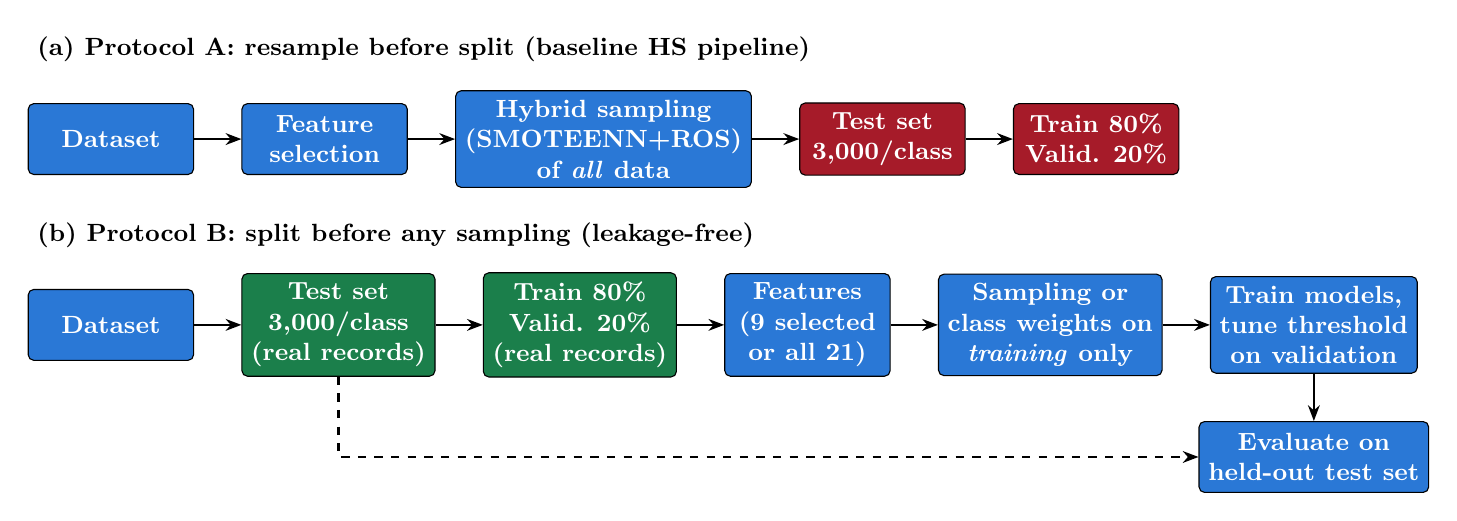
\begin{tikzpicture}[
  node distance=5mm and 6mm,
  box/.style={draw, rounded corners=2pt, fill=boxblue, text=white,
              font=\small\bfseries, align=center, minimum height=9mm,
              minimum width=21mm},
  data/.style={box, fill=boxred},
  good/.style={box, fill=boxgreen},
  arr/.style={-{Stealth[length=2mm]}, thick},
  lbl/.style={font=\small\bfseries, anchor=west}]
  % Protocol A
  \node[lbl] (la) at (0,0) {(a) Protocol A: resample before split (baseline HS pipeline)};
  \node[box, below=4mm of la.south west, anchor=north west] (a1) {Dataset};
  \node[box, right=of a1] (a2) {Feature\\selection};
  \node[box, right=of a2] (a3) {Hybrid sampling\\(SMOTEENN+ROS)\\of \emph{all} data};
  \node[data, right=of a3] (a4) {Test set\\3,000/class};
  \node[data, right=of a4] (a5) {Train 80\%\\Valid. 20\%};
  \draw[arr] (a1) -- (a2); \draw[arr] (a2) -- (a3); \draw[arr] (a3) -- (a4);
  \draw[arr] (a4) -- (a5);
  % Protocol B
  \node[lbl, anchor=west] (lb) at ([yshift=-6mm]la.west |- a3.south) {(b) Protocol B: split before any sampling (leakage-free)};
  \node[box, below=4mm of lb.south west, anchor=north west] (b1) {Dataset};
  \node[good, right=of b1] (b2) {Test set\\3,000/class\\(real records)};
  \node[good, right=of b2] (b3) {Train 80\%\\Valid. 20\%\\(real records)};
  \node[box, right=of b3] (b3f) {Features\\(9 selected\\or all 21)};
  \node[box, right=of b3f] (b4) {Sampling or\\class weights on\\\emph{training} only};
  \node[box, right=of b4] (b5) {Train models,\\tune threshold\\on validation};
  \draw[arr] (b1) -- (b2); \draw[arr] (b2) -- (b3); \draw[arr] (b3) -- (b3f);
  \draw[arr] (b3f) -- (b4); \draw[arr] (b4) -- (b5);
  \node[box, below=6mm of b5] (b6) {Evaluate on\\held-out test set};
  \draw[arr] (b5) -- (b6);
  \draw[arr, dashed] (b2.south) |- (b6.west);
\end{tikzpicture}}
\caption{Overview of the methodology and the two evaluation protocols. (a)
In the resample-before-split protocol of the baseline HS pipeline, synthetic,
duplicated and cleaned records are created before the test set is drawn.
(b) In the leakage-free protocol, used for the baseline HS models (nine
selected features, hybrid sampling) and for the improved pipeline (all 21
features, class weights), the test and validation sets contain only real
records that are never resampled or seen during training.}
\label{fig:method}
\end{figure}

\subsection{Data Collection}

The dataset employed in this study was sourced from Kaggle~\cite{teboul}, a
publicly accessible data repository. It is a refined version of the data
originally compiled by the Behavioral Risk Factor Surveillance System
(BRFSS)~\cite{brfss}. The dataset consists of 253,680 records, each
representing responses from the 2015 BRFSS survey conducted by the Centers
for Disease Control and Prevention (CDC). It includes 22 columns, one of
which is the target variable, ``HeartDiseaseorAttack''. This binary target
variable indicates whether a respondent has ever been told they had coronary
heart disease or a heart attack, where ``0'' signifies no history of coronary heart disease (CHD) or myocardial
infarction (MI) and ``1'' indicates a reported history of CHD or MI. The raw
data comprise 229,787 records without heart disease and 23,893 records with
heart disease. A comprehensive description of the dataset, including the
variables and their corresponding measurements, is provided in
Table~\ref{tab:vars}~\cite{brfsscalc}.

\begin{table}[t]
\centering
\caption{Description of Dataset Variables}
\label{tab:vars}
\small
\begin{tabular}{p{0.3\linewidth}p{0.62\linewidth}}
\toprule
Variable & Description \\
\midrule
HeartDiseaseorAttack & 0 = No history of coronary heart disease (CHD) or myocardial infarction (MI); 1 = Reported CHD or MI \\
HighBP & 0 = No high blood pressure; 1 = High blood pressure \\
HighChol & 0 = No high cholesterol; 1 = High cholesterol \\
CholCheck & 0 = No cholesterol check in past 5 years; 1 = Checked cholesterol in past 5 years \\
BMI & Body Mass Index [12--98] \\
Smoker & 0 = Smoked fewer than 100 cigarettes in lifetime; 1 = Smoked at least 100 cigarettes in lifetime \\
Stroke & 0 = Has never experienced a stroke; 1 = Has experienced a stroke \\
Diabetes & 0 = Absence of diabetes; 1 = Prediabetes / borderline; 2 = Presence of diabetes \\
PhysActivity & 0 = No physical activity or exercise in prior month; 1 = Engaged in physical activity or exercise in prior month \\
Fruits & 0 = Consumes fruit less than once per day; 1 = Consumes fruit one or more times per day \\
Veggies & 0 = Consumes vegetables less than once per day; 1 = Consumes vegetables one or more times per day \\
HvyAlcoholConsump & Adult men: $\geq$14 drinks/week; Adult women: $\geq$7 drinks/week (0 = No, 1 = Yes) \\
AnyHealthcare & Health care coverage / health insurance (0 = No, 1 = Yes) \\
NoDocbcCost & Could not see doctor due to cost in past 12 months (0 = No, 1 = Yes) \\
GenHlth & General health rating: [1, 2, 3] = Excellent, Very Good, Good; [4, 5] = Fair, Poor \\
MentHlth & Days of poor mental health in past 30 days [0--30] \\
PhysHlth & Days of physical illness or injury in past 30 days [0--30] \\
DiffWalk & Serious difficulty walking or climbing stairs (0 = No, 1 = Yes) \\
Sex & 0 = Female, 1 = Male \\
Age & 13-level category: 1 = 18--24, 2 = 25--29, 3 = 30--34, 4 = 35--39, 5 = 40--44, 6 = 45--49, 7 = 50--54, 8 = 55--59, 9 = 60--64, 10 = 65--69, 11 = 70--74, 12 = 75--79, 13 = 80 or older \\
Education & [1, 2, 3] = Did not graduate high school; 4 = High school graduate; 5 = Attended college or technical school; 6 = College graduate \\
Income & 1, 2 = Lower than \$15,000; 3, 4 = \$15,000 to less than \$25,000; 5 = \$25,000 to less than \$35,000; 6 = \$35,000 to less than \$50,000; 7, 8 = \$50,000 or more \\
\bottomrule
\end{tabular}
\end{table}

\subsection{Data Preprocessing}

The dataset is loaded with the pandas library and explored before
modelling. Duplicate entries are removed to
maintain data integrity, leaving 229,781 unique records with 22 columns.
The presence of missing data is assessed, and the analysis confirms that no
missing values exist. The target variable is strongly imbalanced: the
dataset comprises 23,717 cases of heart disease (10.3\%) and 206,064
instances of individuals without heart disease.

Fig.~\ref{fig:dist}(a) depicts the distribution of the target variable and,
among the heart disease cases, the proportions of individuals who have had a
stroke (16.6\%) or who smoke (62.0\%). The age distribution of individuals
with and without heart disease is compared in Fig.~\ref{fig:age}(a); the
prevalence of heart disease increases steeply with age. Panels (b) of both
figures show the data after hybrid sampling and are discussed in
Section~\ref{sec:hs}.

\begin{figure}[t]
\centering
\begin{subfigure}{\linewidth}
  \centering
  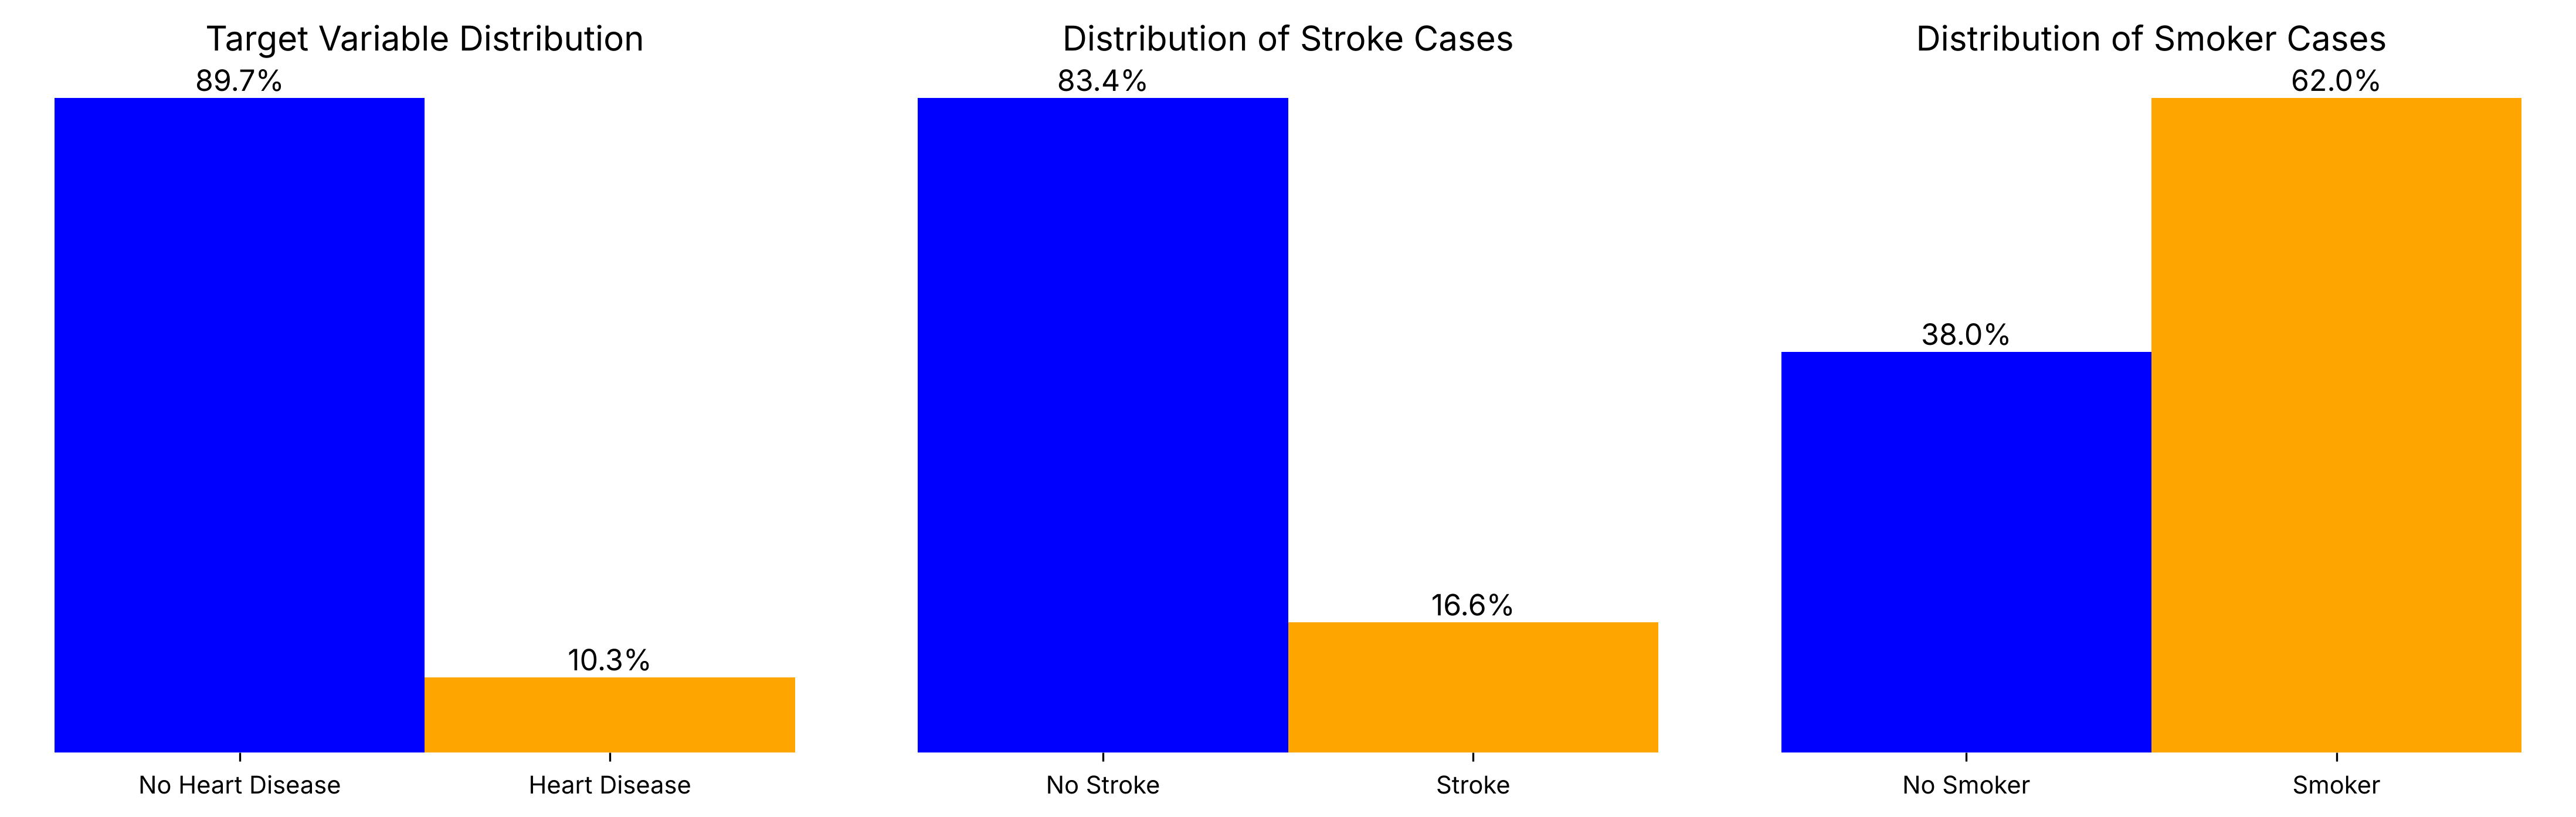
\includegraphics[width=0.9\linewidth]{figures/fig2_distribution_before_sampling.png}
  \caption{Before sampling}
\end{subfigure}
\begin{subfigure}{\linewidth}
  \centering
  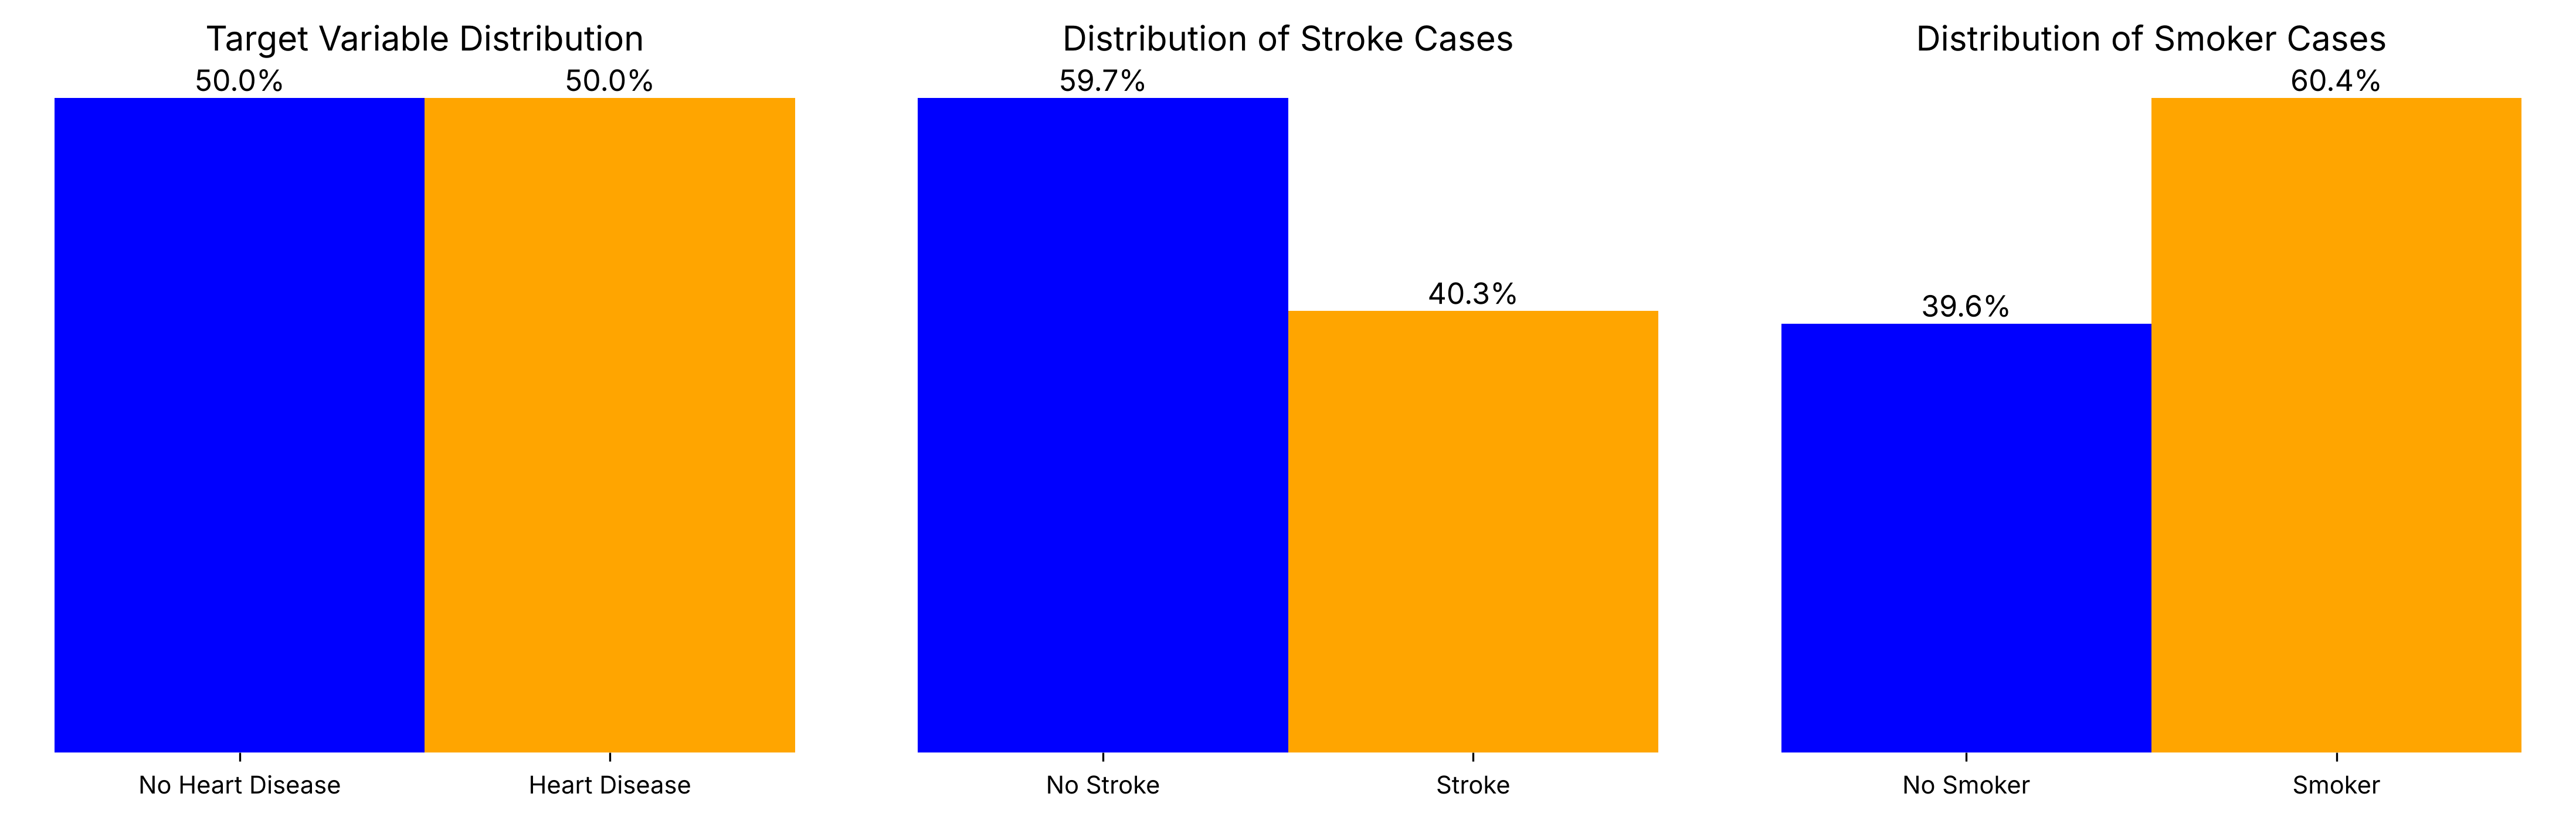
\includegraphics[width=0.9\linewidth]{figures/fig4_distribution_after_sampling.png}
  \caption{After hybrid sampling of the whole dataset (Protocol A)}
\end{subfigure}
\caption{Distribution of the target variable, and of stroke and smoker cases
among individuals with heart disease, before and after hybrid sampling.}
\label{fig:dist}
\end{figure}

\begin{figure}[t]
\centering
\begin{subfigure}{0.49\linewidth}
  \centering
  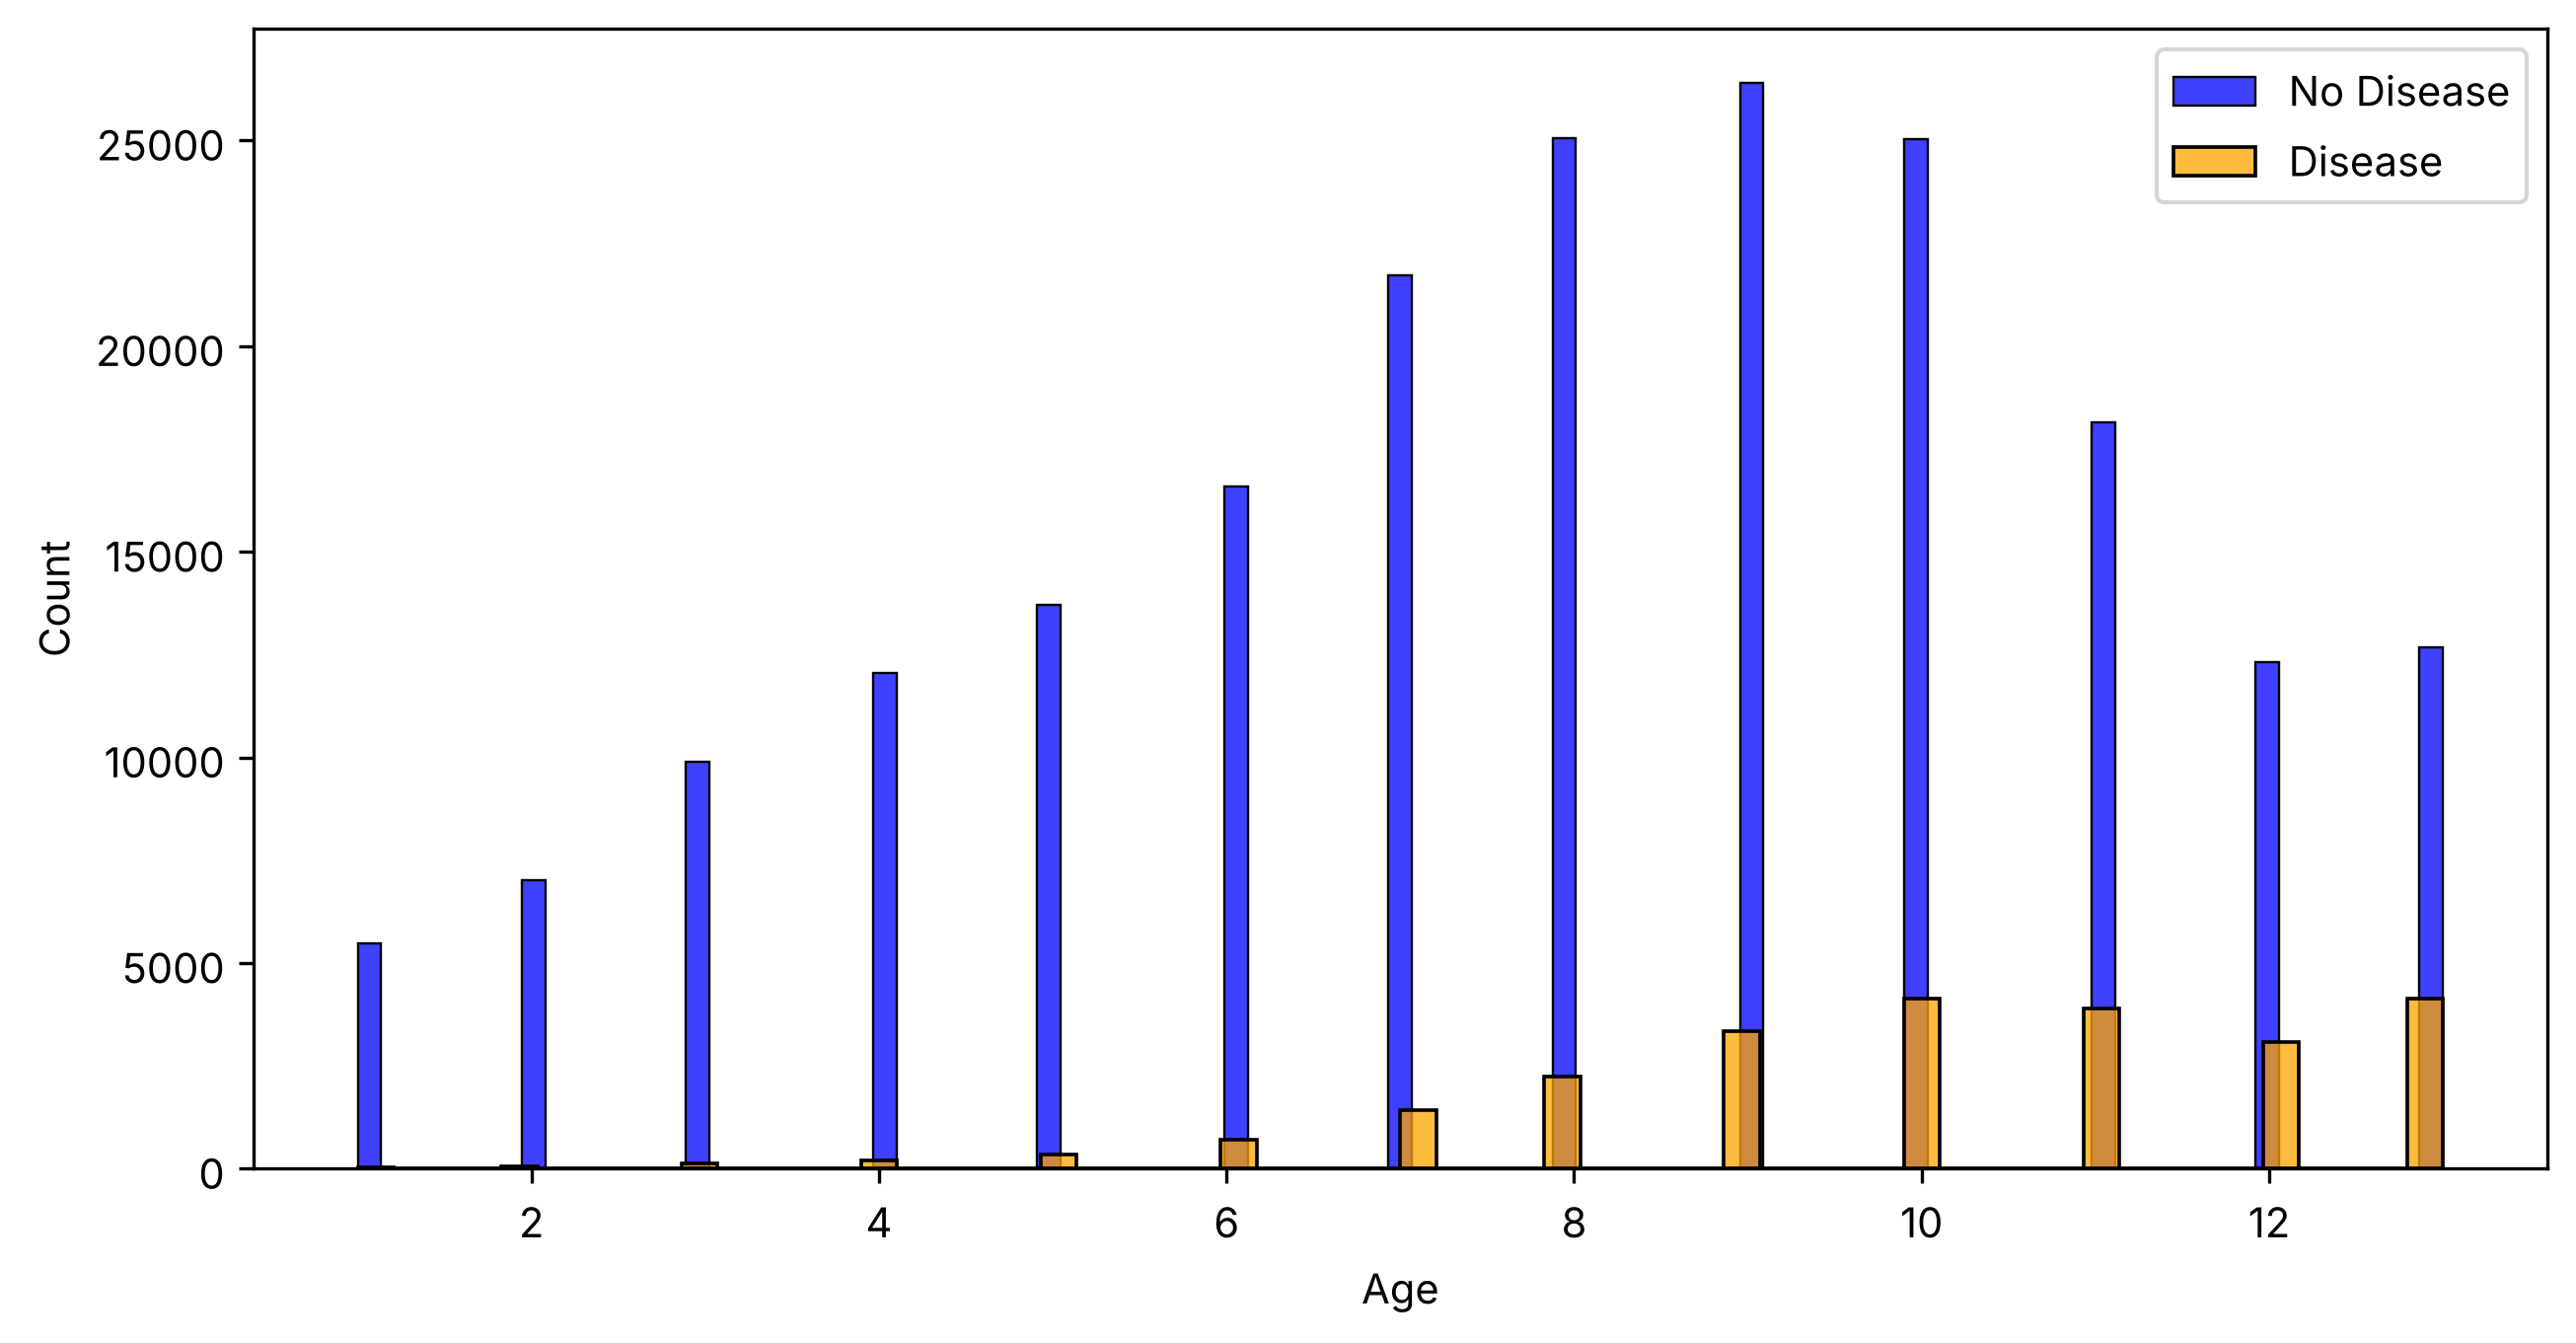
\includegraphics[width=\linewidth]{figures/fig3_age_before_sampling.png}
  \caption{Before sampling}
\end{subfigure}
\begin{subfigure}{0.49\linewidth}
  \centering
  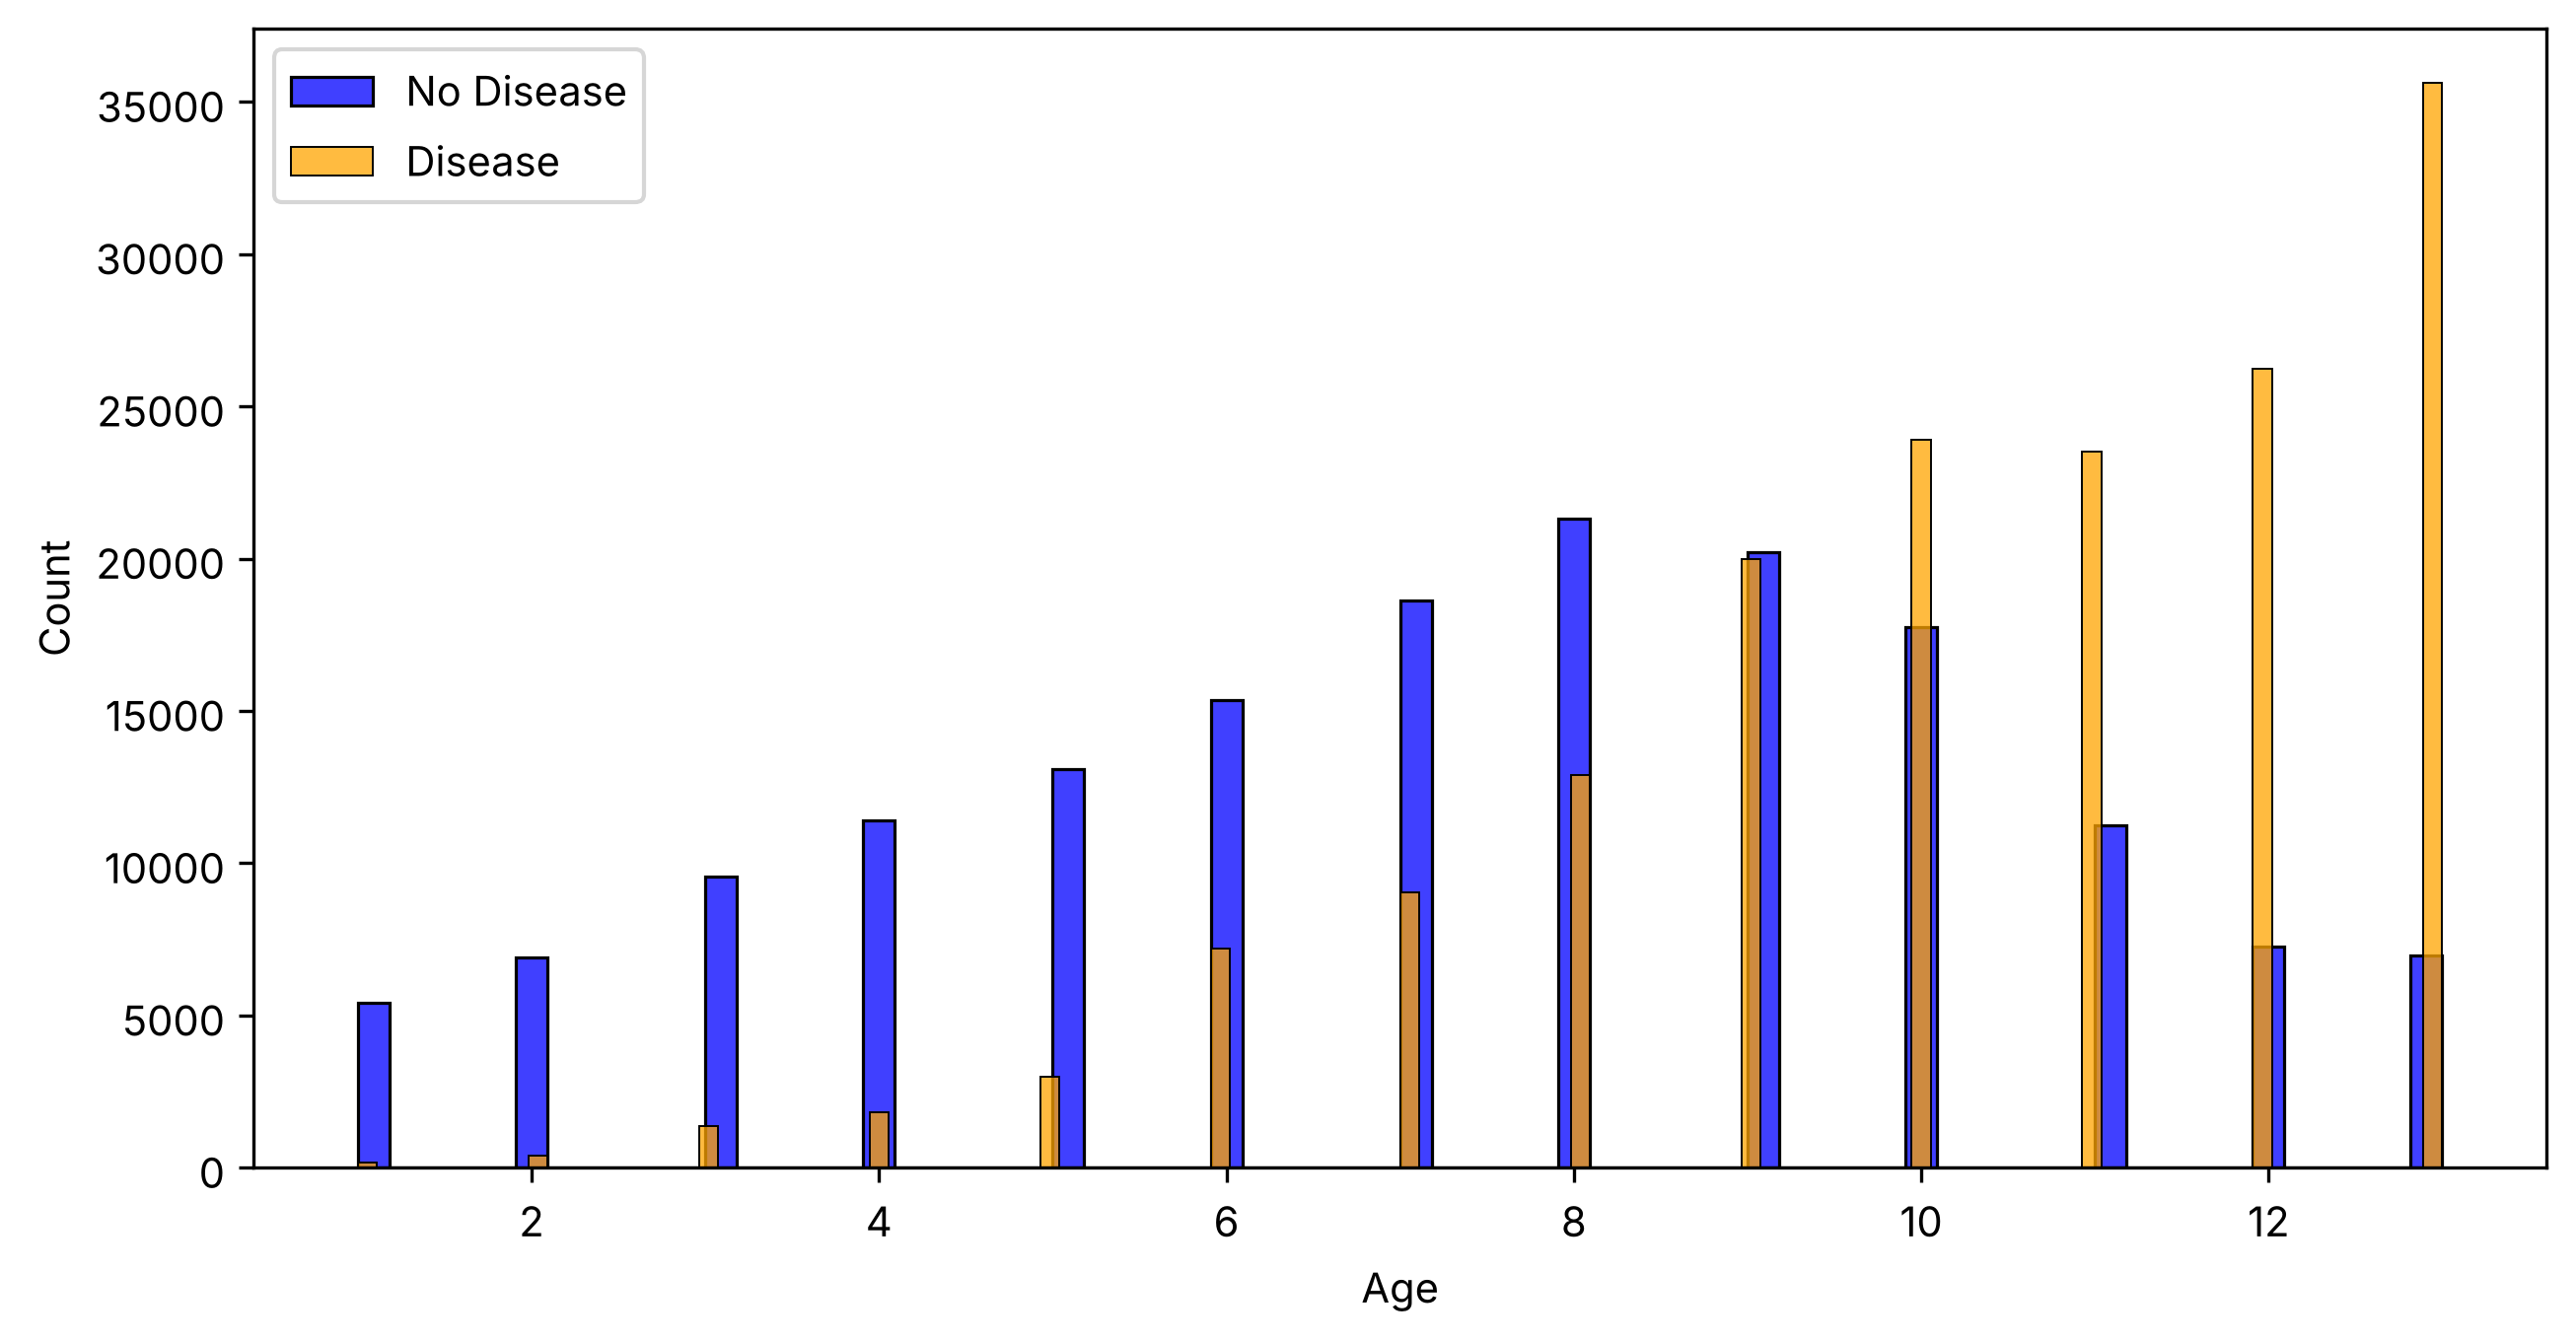
\includegraphics[width=\linewidth]{figures/fig5_age_after_sampling.png}
  \caption{After hybrid sampling (Protocol A)}
\end{subfigure}
\caption{Age distribution of individuals with and without heart disease
before and after hybrid sampling.}
\label{fig:age}
\end{figure}

\subsection{Feature Selection}

Feature selection helps reduce the dataset's complexity while focusing on
the variables most closely linked to the target outcome. A Pearson
correlation matrix is computed and the features are ranked by their
correlation with ``HeartDiseaseorAttack''. The strongest associations are
found for GenHlth ($r = 0.246$), Age (0.224), DiffWalk (0.203), HighBP
(0.201), Stroke (0.199), HighChol (0.176), Diabetes (0.171), PhysHlth
(0.171) and Smoker (0.105). These nine features are used by the baseline
HS models. Because Pearson correlation only
captures linear, univariate association, the improved pipeline
(Section~\ref{sec:improved}) instead uses all 21 features and lets the
models weigh them; the effect of this choice is quantified in the ablation
study.

\subsection{Hybrid Sampling}
\label{sec:hs}

Hybrid sampling combines SMOTEENN with ROS. SMOTE first synthesises new
minority-class instances by interpolating between a minority record and its
nearest minority neighbours until the classes are balanced. ENN then removes
every record whose class disagrees with the majority of its three nearest
neighbours, from both classes. Finally, ROS duplicates minority records
until both classes have equal size. The HS methodology is implemented with
the imbalanced-learn library (random state 42).

Hybrid sampling balances the classes (Fig.~\ref{fig:dist}(b)), but it also
changes who the records describe. Because ENN deletes records that resemble
the opposite class, the remaining heart disease cases are the most
clear-cut ones: among them, the share of individuals who have had a stroke
rises from 16.6\% to 40.3\%. Conversely, the remaining non-CVD records are
younger on average (mean age category 7.85 before and 7.34 after sampling;
Fig.~\ref{fig:age}(b)), consistent with the removal of older healthy
respondents who resemble patients. Section~\ref{sec:results}
shows how these changes affect performance on real patients.

\subsection{Evaluation Protocols}
\label{sec:protocols}

\paragraph{Protocol A (resample before split).} This protocol, common in
published pipelines, is used by the baseline HS pipeline. HS is applied to the whole dataset, which yields 330,288
records (165,144 per class). From this resampled dataset 3,000 records per
class are drawn at random as the test set; the remaining records are split
80/20 into training (259,430) and validation (64,858) sets. Five-fold
cross-validation is likewise run on the resampled data.

\paragraph{Protocol B (split before sampling, leakage-free).} Before any
sampling, 3,000 \emph{real} records per class are drawn from the deduplicated
dataset as the test set. The remaining records are split, stratified by
class, into training (179,024 records, 80\%) and validation (44,757 records,
20\%) sets. Sampling, when used, is applied to the training set only; the
validation and test sets contain only real records with their natural
characteristics. The test set is balanced, so its accuracy equals the
balanced accuracy, which allows a direct comparison with Protocol A. For
cross-validation the 223,781 non-test records are split into five
stratified folds; the held-out fold keeps the real prevalence of about
10.3\%, and any sampling, early stopping and threshold tuning use only the
training folds.

\subsection{Improved Pipeline}
\label{sec:improved}

Motivated by the leakage analysis and the ablation study in
Section~\ref{sec:results}, we propose an improved pipeline that is
evaluated under Protocol B. It makes four changes to the baseline HS
pipeline:
\begin{enumerate}
  \item \textbf{All 21 features} are used instead of the nine
    correlation-selected ones.
  \item \textbf{Class weighting replaces resampling.} The models are
    trained on the real, imbalanced training data; errors on the minority
    class are weighted by the inverse class frequency
    (\texttt{class\_weight="balanced"} for DT, SVM, LR and the DL models;
    \texttt{scale\_pos\_weight} $=$ 9.8, the ratio of negative to positive training records, for XGBoost).
  \item \textbf{Regularised models.} The DT is limited to a depth of 8 with
    at least 50 records per leaf; XGBoost uses shallow trees (depth 5),
    learning rate 0.03, row and column subsampling of 0.8 and early
    stopping on the validation AUC (patience 100 rounds, at most 2,000
    trees); the DL models use early stopping on the validation loss
    (patience 3, at most 30 epochs, batch size 256) and restore the best
    weights. Logistic regression (LR) is added as an interpretable baseline.
  \item \textbf{Decision threshold tuned on the validation set.} Instead of
    the default threshold of 0.5, the threshold that maximises Youden's
    index $J = \text{sensitivity} + \text{specificity} - 1$ on the
    validation set is used.
\end{enumerate}

\subsection{External Evaluation on Clinical Data}
\label{sec:cleveland}

Most published CVD studies use the UCI Cleveland heart disease
data~\cite{detrano}, 303 hospital patients described by 13 clinical
measurements, including chest-pain type, resting ECG, maximum exercise heart
rate, exercise-induced ST depression and thallium scintigraphy. To compare
with these studies on equal terms, the improved pipeline is applied,
unchanged, to this dataset (PMLB version~\cite{pmlb}). The 6 patients with
missing values are removed, leaving 297, of whom 137 have heart disease, and
the categorical variables are one-hot encoded. Because a single split of
such a small dataset yields test sets of about 60 patients, the models are
evaluated with five repetitions of stratified five-fold cross-validation; in
every fold, early stopping and threshold tuning use only the training
portion.

\section{DL AND ML ARCHITECTURE ANALYSIS}
\label{sec:arch}

\subsection{ML Models}

\paragraph{Decision Tree.} A DT classifier (C4.5-style, entropy splitting
criterion) learns a hierarchy of feature tests that map input features to
the CVD label. In the HS pipeline the tree is grown to full depth.

\paragraph{SVM.} An SVM classifier with a linear kernel separates the two
classes with a maximum-margin hyperplane. Features are min--max scaled, and
the model is fitted with the LIBLINEAR solver, which solves the same linear
SVM problem as a kernel SVM with a linear kernel but scales to several
hundred thousand records. Its decision values are used to compute the ROC
curve.

\paragraph{XGBoost.} XGBoost builds an ensemble of gradient-boosted trees,
each correcting the errors of the previous ones. The HS pipeline uses the
library defaults.

\paragraph{Logistic regression.} LR models the log-odds of CVD as a linear
function of the standardised features. It is used only in the improved
pipeline, as an interpretable baseline.

The settings of all models in the improved pipeline (class weights, depth
limit, early stopping and threshold tuning) are given in
Section~\ref{sec:improved}.

\subsection{DL Models}

All DL models share a preprocessing stage: features are min--max scaled and
passed through an autoencoder whose encoder (one dense layer of 64 ReLU
units, trained for 10 epochs to reconstruct its input with a sigmoid output
layer and mean-squared-error loss) produces a 64-dimensional representation
that is fed to the classifier. The classifiers are:
\begin{itemize}
  \item \textbf{CNN}: Conv1D (8 filters, kernel size 2, ReLU) $\rightarrow$
    max pooling (2) $\rightarrow$ flatten $\rightarrow$ dense (16, ReLU)
    $\rightarrow$ dense (1, sigmoid); 20 epochs.
  \item \textbf{NN}: dense (64, ReLU) $\rightarrow$ dense (32, ReLU)
    $\rightarrow$ dense (1, sigmoid); 10 epochs.
  \item \textbf{MLP}: dense (128) $\rightarrow$ dense (64) $\rightarrow$
    dense (32), all ReLU $\rightarrow$ dense (1, sigmoid); 20 epochs.
\end{itemize}
All DL models are trained with the Adam optimiser and binary cross-entropy
loss, with a batch size of 32 in the HS pipeline.

\subsection{Evaluation Metrics}

For performance evaluation, a confusion matrix is employed to analyze the
results of each model. The matrix produces four key metrics: true positives
(TP), true negatives (TN), false positives (FP), and false negatives (FN).
These metrics facilitate the computation of additional performance
indicators.

\begin{enumerate}
\item Accuracy: the proportion of correct predictions~\cite{ullah2022}:
\begin{equation}
\text{Accuracy} = \frac{TP + TN}{TP + TN + FP + FN}
\end{equation}
\item Precision (positive predictive value): the proportion of predicted CVD
cases that are correct~\cite{ullah2023}:
\begin{equation}
\text{Precision} = \frac{TP}{TP + FP}
\end{equation}
\item Recall (sensitivity): the proportion of actual CVD cases that are
detected~\cite{ullah2023}:
\begin{equation}
\text{Recall} = \frac{TP}{TP + FN}
\end{equation}
\item F1-score: the harmonic mean of precision and recall~\cite{ullah2022}:
\begin{equation}
\text{F1-score} = \frac{2 \cdot (\text{Precision} \cdot \text{Recall})}{\text{Precision} + \text{Recall}}
\end{equation}
\item Area Under the Curve (AUC): the area under the receiver operating
characteristic (ROC) curve, which traces the true positive rate (TPR) against
the false positive rate (FPR) across classification
thresholds~\cite{ullah2022}. The AUC ranges from 0.5 (random guessing) to 1.0
(perfect classification) and is computed from the continuous model scores:
\begin{equation}
\text{AUC} = \int_0^1 \text{TPR}(\text{FPR})\, d(\text{FPR})
\end{equation}
\end{enumerate}

Unlike accuracy, precision and F1, the AUC does not depend on the decision
threshold or on the class balance of the test set, which makes it the most
robust metric for comparing models across protocols.

\section{RESULTS AND DISCUSSION}
\label{sec:results}

The results are presented in four steps. Section~\ref{sec:resA} reports
the performance of the HS models under the resample-before-split protocol
(Protocol A). Section~\ref{sec:leak} analyses why these results do not
transfer to new patients. Section~\ref{sec:resB} evaluates the same models
and the improved pipeline on real, held-out records (Protocol B), including
an ablation study and five-fold cross-validation, and
Section~\ref{sec:compare} compares the findings with existing studies. All
experiments use a fixed random state of 42 and can be reproduced with the
released code.

\subsection{Performance under the Resample-Before-Split Protocol}
\label{sec:resA}

Table~\ref{tab:protoA} reports the test-set performance of all models when
the full dataset is resampled before it is split (Protocol A), as in the
original pipeline. With hybrid sampling every model appears highly
accurate: the DT reaches 99.78\% accuracy and 100\% recall, XGBoost
98.23\%, the MLP 98.45\% and the CNN and NN 96.02\% and 94.70\%; the ROC
curves (Fig.~\ref{fig:rocA}) hug the top-left corner with AUC values of
0.96--1.00. Models trained with ROS alone, in contrast, reach only about
75.5\% accuracy and an AUC of 0.83. The last column lists the accuracies
reported in the original version of this study; our reimplementation
reproduces them closely for HS and ROS. For SMOTEENN alone our
reimplementation obtains higher values than originally reported (88.6--91.2\%
vs.\ 74--75\%), consistent with the effect of ENN cleaning on the test set
discussed in Section~\ref{sec:leak}.

\begin{table}[t]
\centering
\caption{Test performance under Protocol A (resample before split; 3,000
test records per class drawn from the resampled data). Last column:
accuracy reported in the original version of this study.}
\label{tab:protoA}
\small
\begin{tabular}{llcccccc}
\toprule
Sampling & Model & Acc. (\%) & Prec. (\%) & Rec. (\%) & F1 (\%) & AUC (\%) & Orig. Acc. (\%) \\
\midrule
\multirow{3}{*}{SMOTEENN} & CNN & 88.58 & 96.81 & 79.80 & 87.48 & 98.08 & 74.09 \\
 & NN & 89.18 & 96.41 & 81.40 & 88.27 & 98.38 & 75.08 \\
 & MLP & 91.15 & 97.72 & 84.27 & 90.50 & 99.12 & 75.00 \\
\midrule
\multirow{3}{*}{ROS} & CNN & 75.55 & 72.70 & 81.83 & 77.00 & 83.17 & 75.13 \\
 & NN & 75.47 & 72.63 & 81.73 & 76.91 & 83.20 & 75.51 \\
 & MLP & 75.63 & 72.39 & 82.87 & 77.28 & 83.30 & 75.91 \\
\midrule
\multirow{6}{*}{HS} & CNN & 96.02 & 93.13 & 99.37 & 96.15 & 98.73 & 93.01 \\
 & NN & 94.70 & 94.49 & 94.93 & 94.71 & 98.63 & 95.96 \\
 & MLP & 98.45 & 97.12 & 99.87 & 98.47 & 99.47 & 97.55 \\
 & DT & 99.78 & 99.57 & 100.00 & 99.78 & 99.78 & 99.70 \\
 & SVM & 89.57 & 88.79 & 90.57 & 89.67 & 95.96 & 93.16 \\
 & XGBoost & 98.23 & 96.80 & 99.77 & 98.26 & 99.65 & 97.80 \\
\bottomrule
\end{tabular}
\end{table}

\begin{figure}[t]
\centering
\begin{subfigure}{0.49\linewidth}
  \centering
  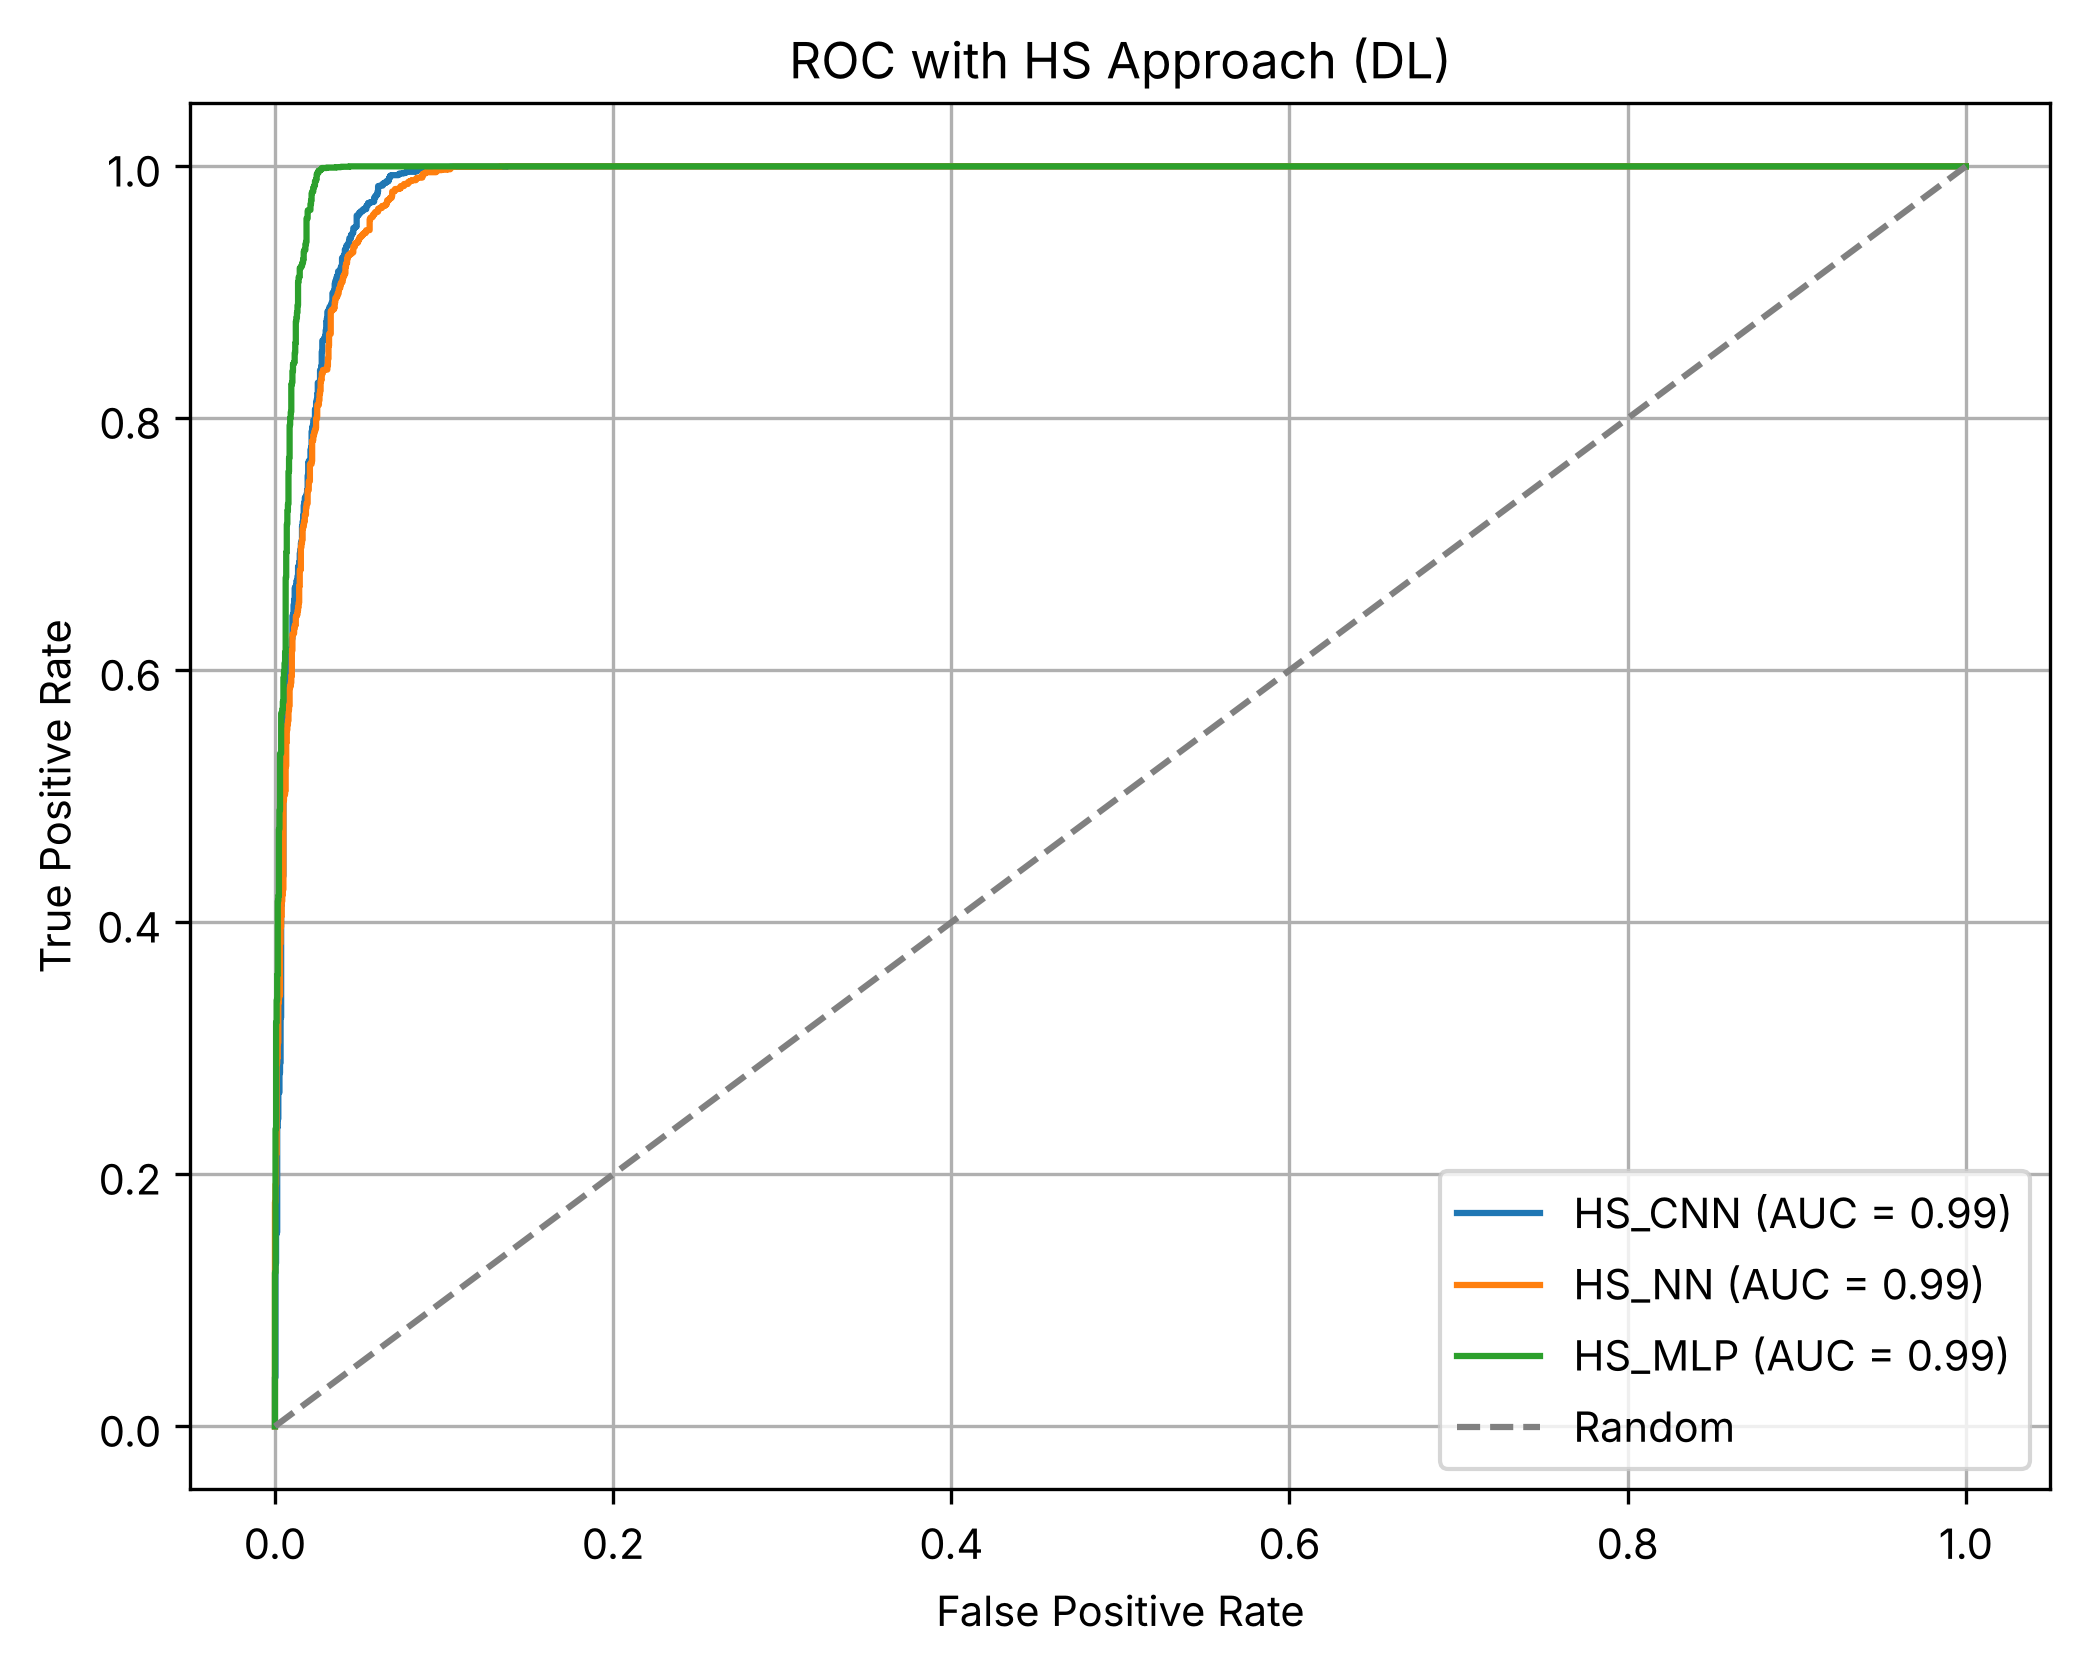
\includegraphics[width=\linewidth]{figures/roc_hs_dl.png}
  \caption{HS with DL models}
\end{subfigure}
\begin{subfigure}{0.49\linewidth}
  \centering
  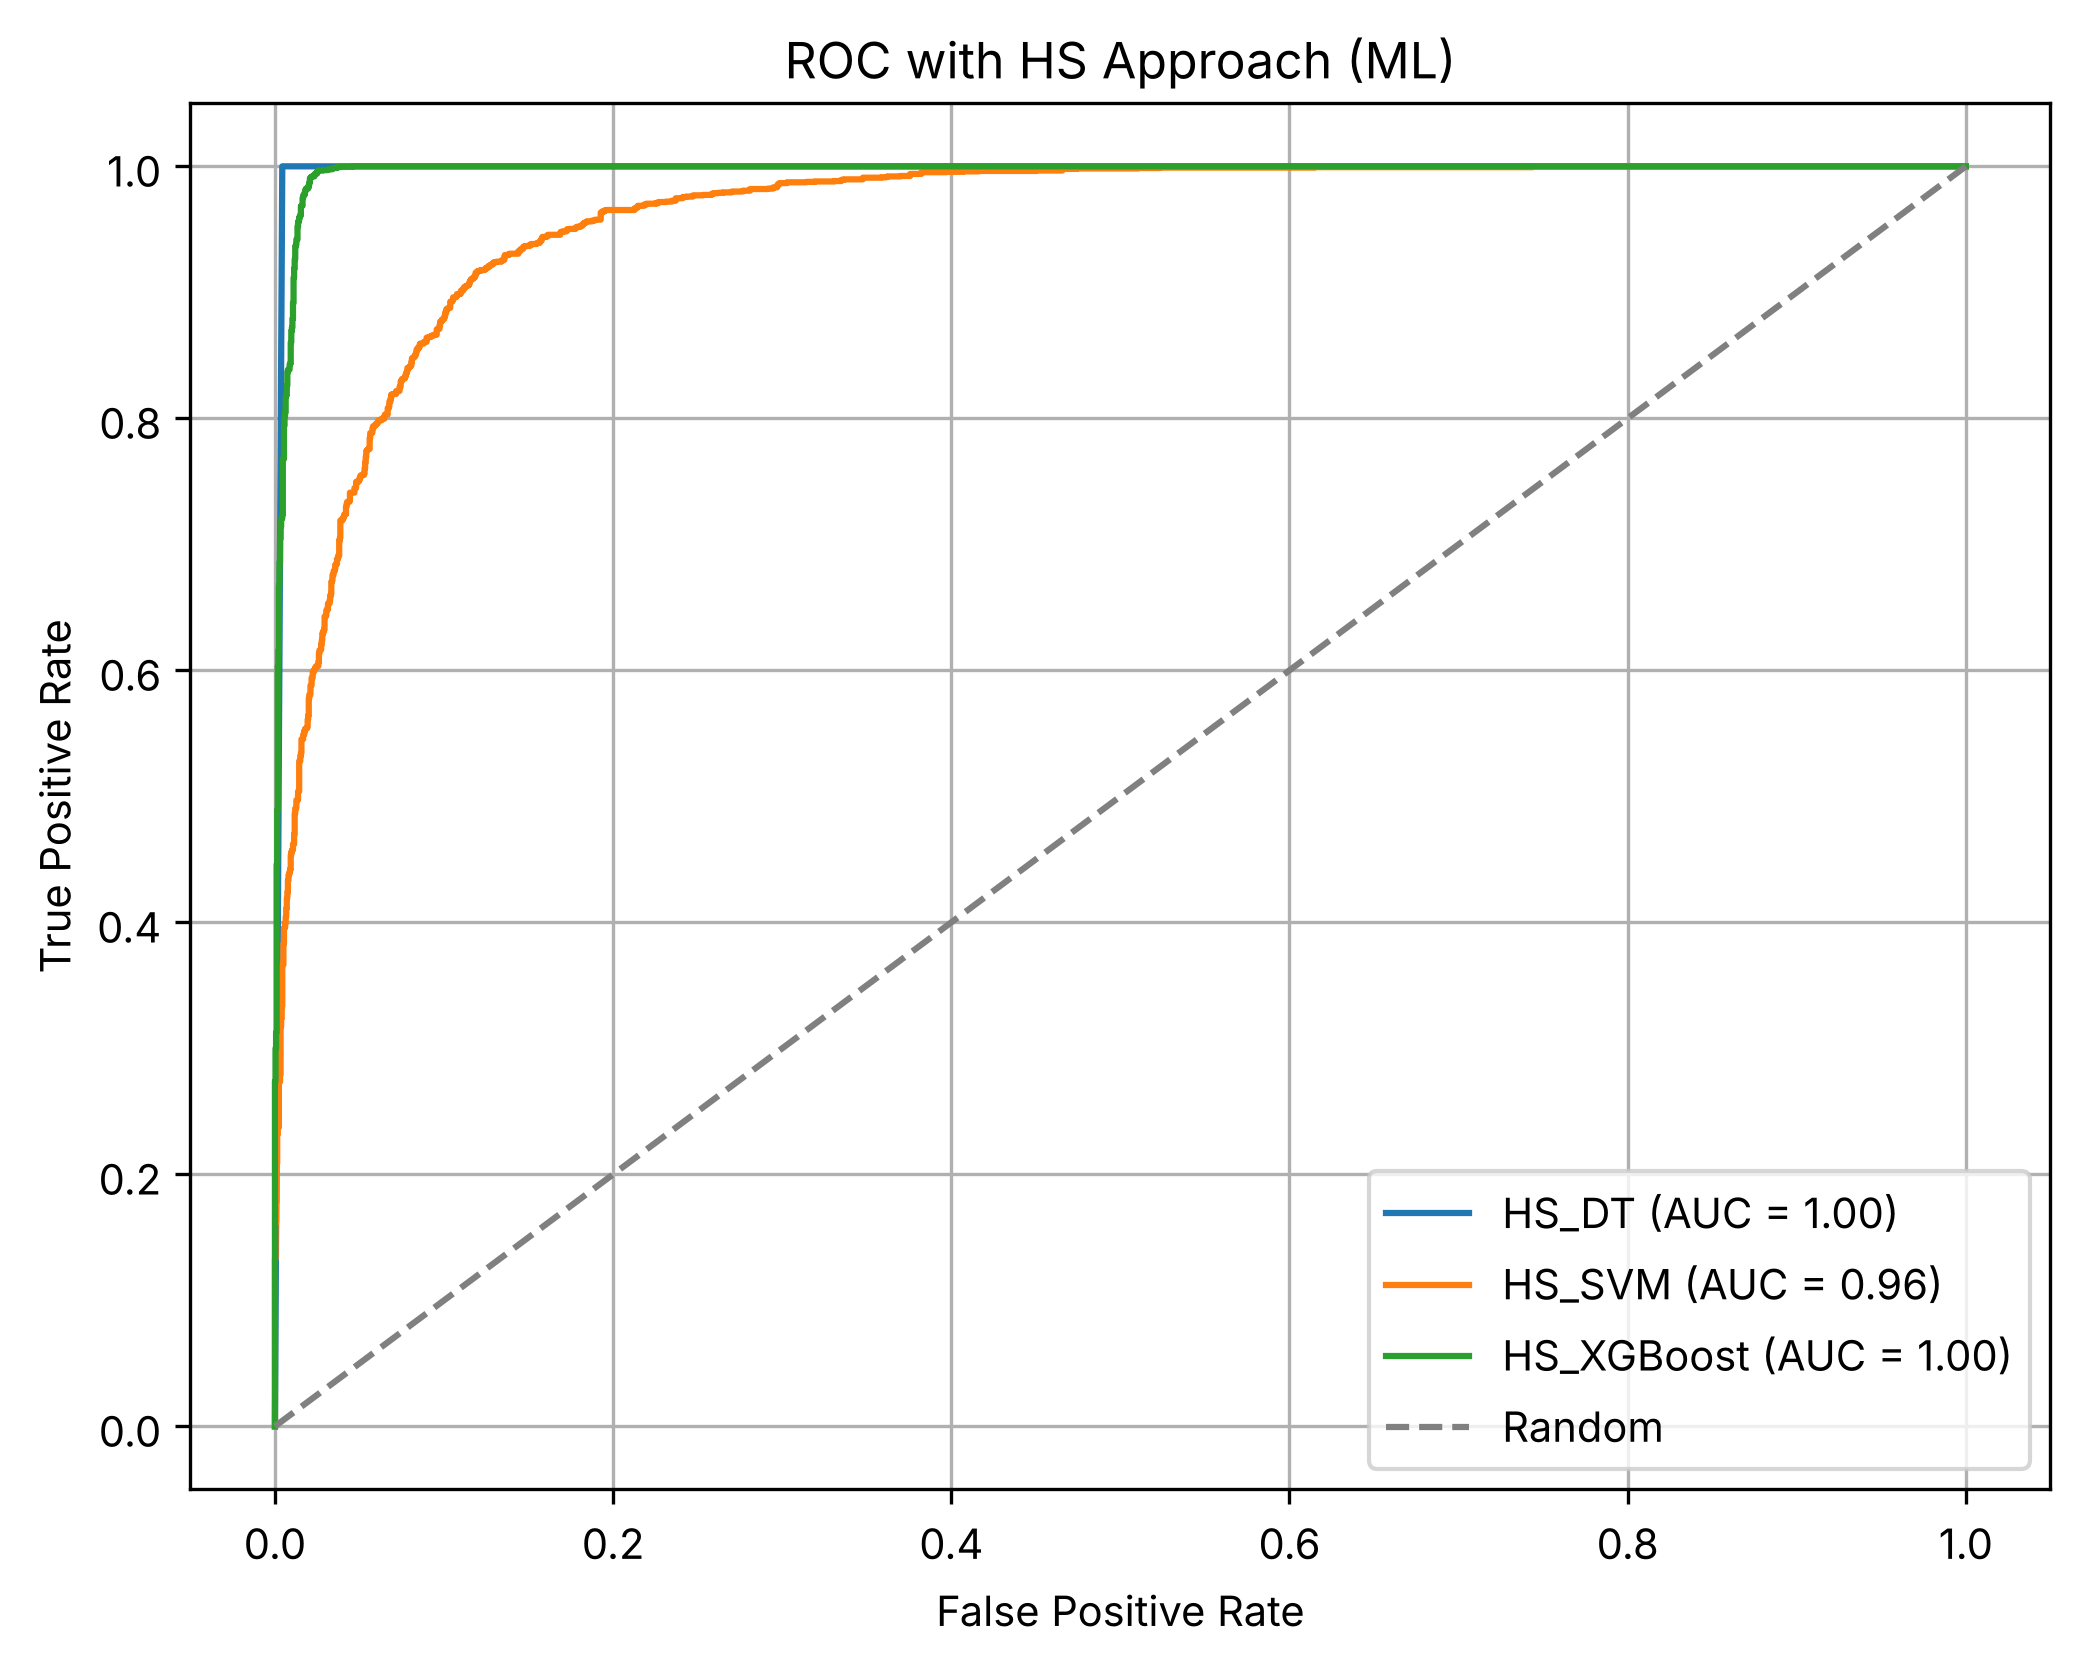
\includegraphics[width=\linewidth]{figures/roc_hs_ml.png}
  \caption{HS with ML models}
\end{subfigure}
\caption{ROC curves under Protocol A (resample before split). The
near-perfect curves are an artefact of data leakage
(Section~\ref{sec:leak}).}
\label{fig:rocA}
\end{figure}

\subsection{Data Leakage in the Resample-Before-Split Protocol}
\label{sec:leak}

Two properties of HS explain why the Protocol A results overstate how the
models would perform on new patients.

\paragraph{Duplication.} SMOTE first creates 182,347 synthetic positive
records to balance the classes. ENN then removes most of the positive
records together with 40,920 real negative records, leaving 22,239
positive and 165,144 negative records. ROS finally
duplicates each remaining positive record about 7.4 times on average to
balance the classes. When the test set is drawn from these data, its
positive records are copies of records that also occur in the training set.
Table~\ref{tab:leak} quantifies this: under Protocol A, 100\% of the
positive test records have an identical record (same features and label) in
the training set, compared with 4.6\% under Protocol B. A fully grown
decision tree can simply memorise these records, which explains its
near-perfect score.

\paragraph{Cleaning of the test population.} ENN removes every record whose
label disagrees with most of its nearest neighbours. These are exactly the
patients whose survey answers look like those of the opposite class: 19.9\%
of all real negative records are deleted before the test set is drawn. The
test set therefore no longer contains the borderline cases that make CVD
prediction from survey data hard, and the classes become artificially
separable. This is why HS raises even the smooth DL models from about
75.5\% (ROS alone, which removes no records) to 94.7--98.5\%. In a clinical
setting such patients cannot be removed.

\begin{table}[t]
\centering
\caption{Overlap between test and training sets for hybrid sampling:
percentage of test records that have an identical record (all nine features
and the label) in the training set. Negative records overlap even without
leakage because healthy respondents often give identical answers to the
nine mostly binary questions.}
\label{tab:leak}
\small
\begin{tabular}{lccc}
\toprule
Protocol & All test records & Positive (CVD) & Negative \\
\midrule
A: resample before split & 98.5\% & 100.0\% & 96.9\% \\
B: split before sampling & 40.9\% & 4.6\% & 77.1\% \\
\bottomrule
\end{tabular}
\end{table}

Both effects are well-documented forms of data
leakage~\cite{kaufman,kapoor}: information about the test data enters
model training or shapes the test data themselves. Santos et
al.~\cite{santos} showed that oversampling before cross-validation produces
over-optimistic estimates, and our results quantify the size of this bias
for CVD prediction: more than 40 percentage points of accuracy for the DT.
The cross-validation results of the original version of this study
(92.7--99.7\% accuracy for the HS models) suffer from the same problem,
because the folds were drawn from the resampled data, and are therefore
replaced by leakage-free cross-validation in Section~\ref{sec:cv}.

\subsection{Performance on Real, Unseen Records}
\label{sec:resB}

\subsubsection{The original HS pipeline under Protocol B}

Table~\ref{tab:protoB} (left) shows the same HS models trained on the
resampled training set and evaluated on 6,000 real records that were held
out before sampling. Performance drops sharply: accuracy falls to
57.4--70.8\% and the AUC to 0.57--0.81. The fully grown DT, the best model
under Protocol A, is close to chance level (AUC 0.574) because the records
it memorised do not recur among new patients. All HS models are also very
conservative on real data: their recall ranges from 18.5\% (DT) to 60.2\%
(SVM), so most CVD cases are missed. Because ENN removed the borderline
negatives from the training data, the models learn that only clear-cut
profiles are negative and place the default decision threshold of 0.5 far
from where it would be on the real population.

\begin{table}[t]
\centering
\caption{Test performance under Protocol B (6,000 real records, 3,000 per
class, held out before any sampling). Left: original HS pipeline (nine
features, hybrid sampling of the training data, threshold 0.5). Right:
improved pipeline (all 21 features, class weights, regularised models,
threshold tuned on the validation set). All values in \%.}
\label{tab:protoB}
\footnotesize
\setlength{\tabcolsep}{3.5pt}
\begin{tabular}{l|ccccc|ccccc}
\toprule
 & \multicolumn{5}{c|}{Original HS pipeline} & \multicolumn{5}{c}{Improved pipeline} \\
Model & Acc. & Prec. & Rec. & F1 & AUC & Acc. & Prec. & Rec. & F1 & AUC \\
\midrule
\inputrows{tables/protocol_b_test.tex}
\bottomrule
\end{tabular}
\end{table}

\subsubsection{Ablation study}

To identify which design choices limit performance on real data, we varied
them one at a time for XGBoost and the DT (Table~\ref{tab:ablation}). The
AUC measures how well a model ranks patients by risk, independently of the
threshold; accuracy is reported both at the default threshold of 0.5 and at
the threshold tuned on the validation set.

\begin{table}[t]
\centering
\caption{Ablation study under Protocol B (real test set). ``Tuned'' denotes
the threshold that maximises Youden's $J$ on the validation set.}
\label{tab:ablation}
\small
\begin{tabular}{llccc}
\toprule
Model & Configuration & AUC (\%) & Acc.\ @ 0.5 (\%) & Acc.\ @ tuned (\%) \\
\midrule
XGBoost & 9 features, HS (original) & 74.31 & 61.58 & 68.28 \\
XGBoost & 9 features, ROS only & 82.06 & 74.35 & 74.25 \\
XGBoost & 9 features, no resampling & 82.25 & 53.27 & 74.55 \\
XGBoost & 21 features, no resampling & 83.54 & 54.75 & 75.25 \\
XGBoost & 21 features, class weights, regularised (improved) & 83.99 & -- & 76.00 \\
\midrule
DT & 9 features, HS, full depth (original) & 57.40 & 57.40 & 57.40 \\
DT & 21 features, class weights, depth 8 (improved) & 82.50 & -- & 74.90 \\
\bottomrule
\end{tabular}
\end{table}

Four findings emerge. First, hybrid sampling is the main cause of the loss:
replacing it with ROS alone raises the AUC of XGBoost from 0.743 to 0.821,
and dropping resampling altogether gives the same AUC (0.823), showing that
synthetic records and ENN cleaning distort the data rather than add
information. Second, without resampling the default threshold of 0.5 is
unsuitable for imbalanced data (53.3\% accuracy, because almost every
record is predicted negative), whereas a threshold tuned on the validation
set restores 74.6\% accuracy; resampling and threshold tuning address the
same problem, but tuning does so without altering the data. Third, using all
21 features instead of the nine correlation-selected ones increases the AUC
from 0.823 to 0.835: features such as sex, income, BMI and education carry
predictive information that a univariate correlation ranking misses.
Fourth, regularisation (shallow, early-stopped boosting and a depth-limited
tree) prevents the models from memorising individual records; it turns the
DT from a near-random classifier into a competitive model (AUC 0.825).

\subsubsection{The improved pipeline}

Table~\ref{tab:protoB} (right) shows that the improved pipeline raises
every model on real, unseen records, and Fig.~\ref{fig:improved}
summarises its results. Accuracy
increases to 74.9--76.0\%, recall to 78.8--82.8\% and the AUC to
0.825--0.840. The largest gains concern recall: the improved XGBoost
detects 82.8\% of CVD cases, compared with 30.5\% for the original HS
XGBoost, and the improved DT detects 78.9\% compared with 18.5\%. The ROC
curves of all improved models nearly coincide (Fig.~\ref{fig:rocB}), and
logistic regression performs on par with XGBoost and the three DL models.
The confusion matrices (Fig.~\ref{fig:cmB}) show a balanced error profile:
the improved XGBoost correctly identifies 2,483 of 3,000 CVD cases and
2,077 of 3,000 non-CVD cases. The learning curves of the DL models
(Fig.~\ref{fig:lcB}) show the validation loss decreasing for about ten
epochs and then levelling off; training stops three epochs after the last
improvement and the best weights are restored, which prevents
over-fitting. The training loss is computed with class weights and is
therefore not directly comparable to the unweighted validation loss.

\begin{figure}[t]
\centering
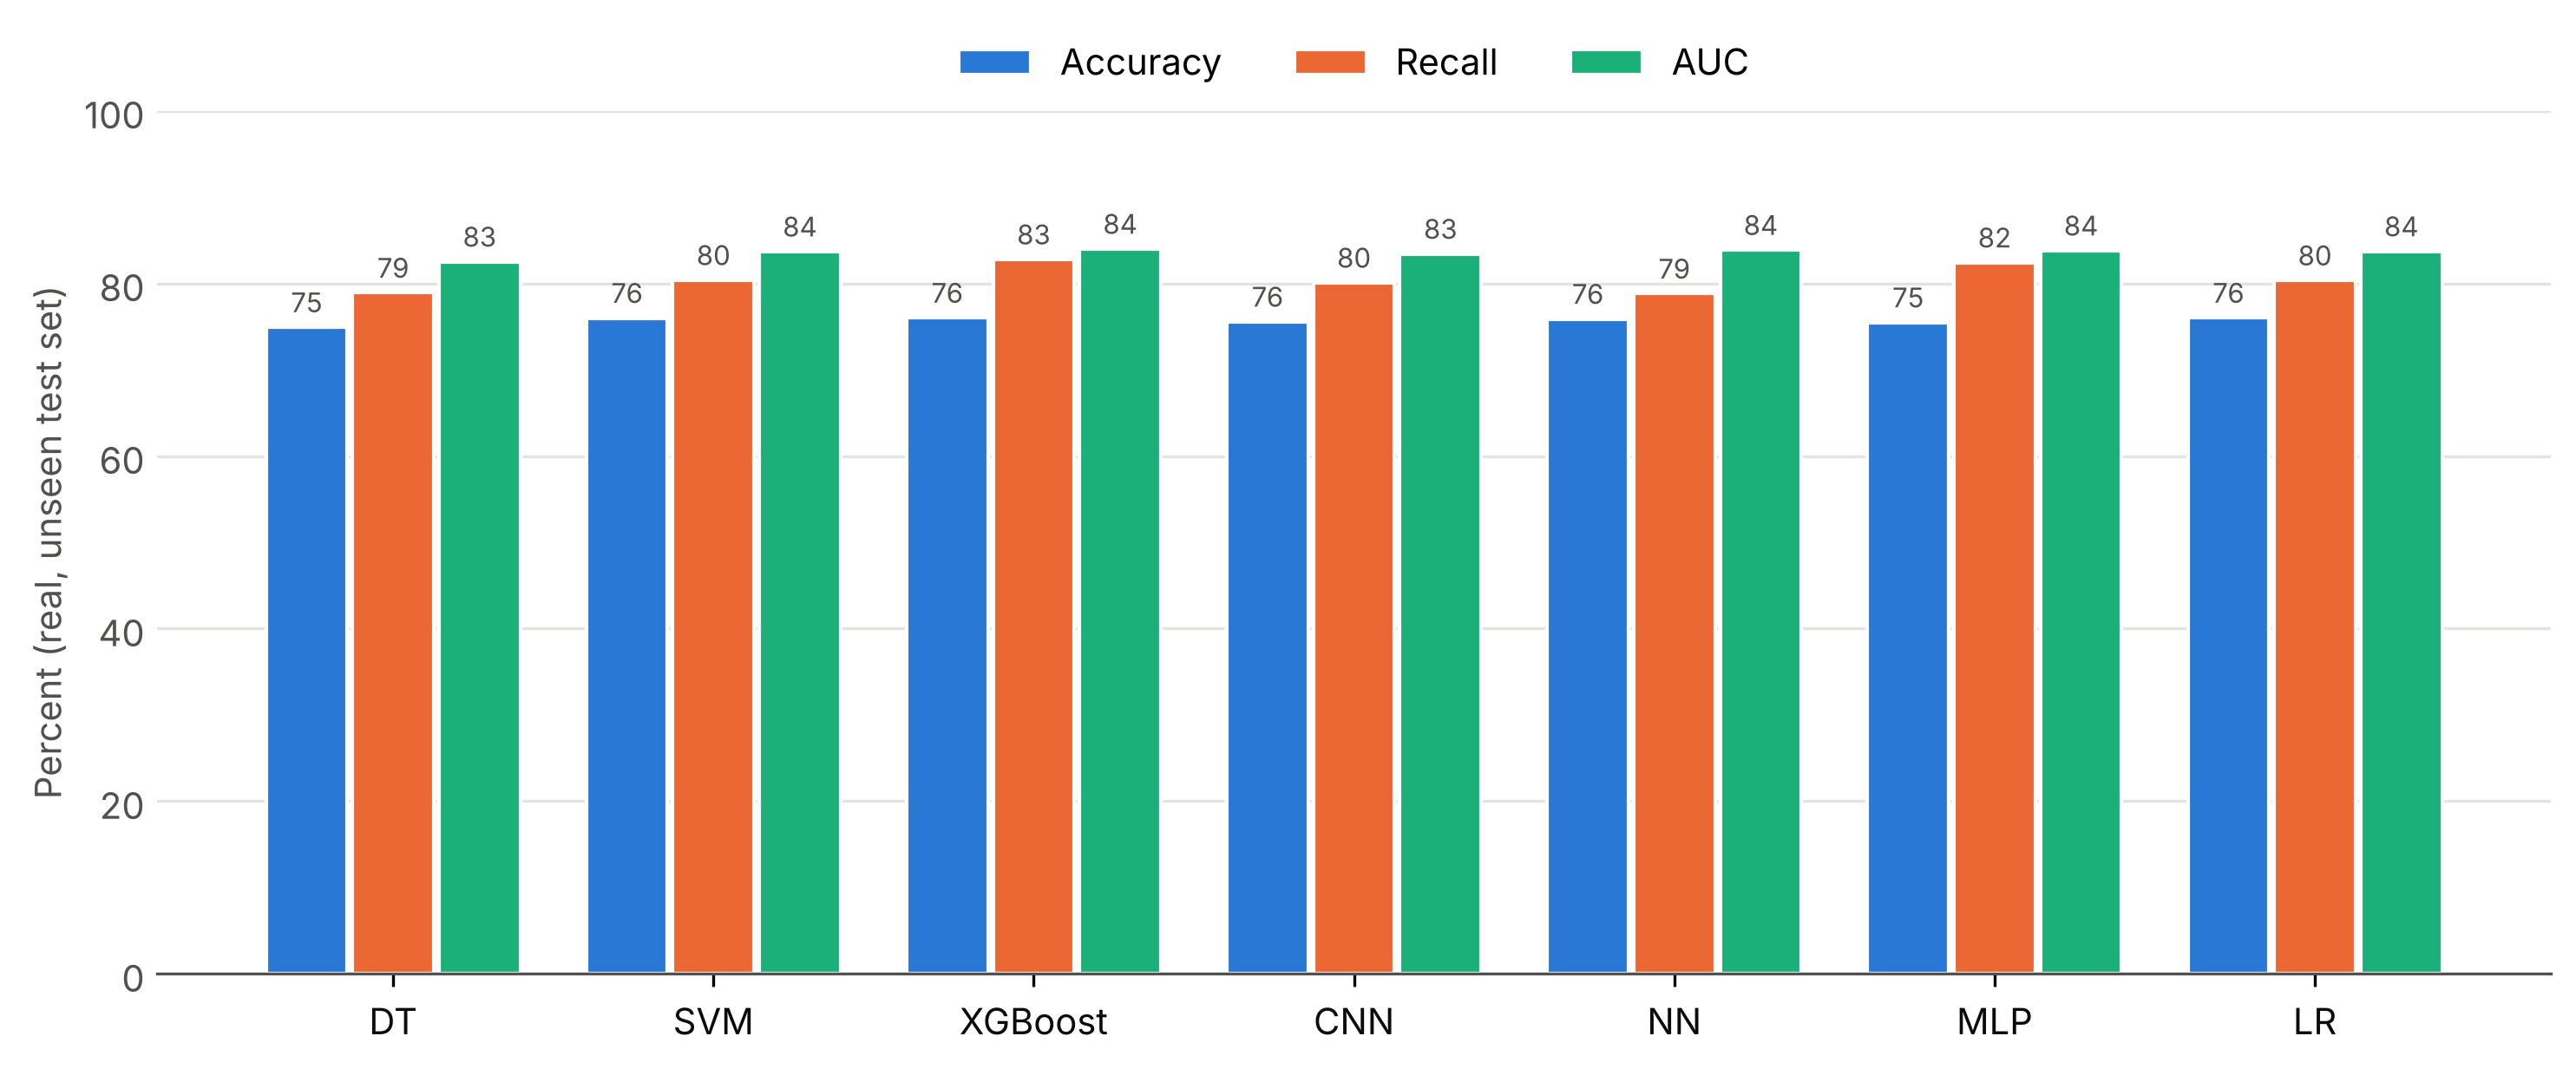
\includegraphics[width=0.9\linewidth]{figures/improved_results.png}
\caption{Accuracy, recall and AUC of the improved models on the real,
unseen test set (Protocol B).}
\label{fig:improved}
\end{figure}

\begin{figure}[t]
\centering
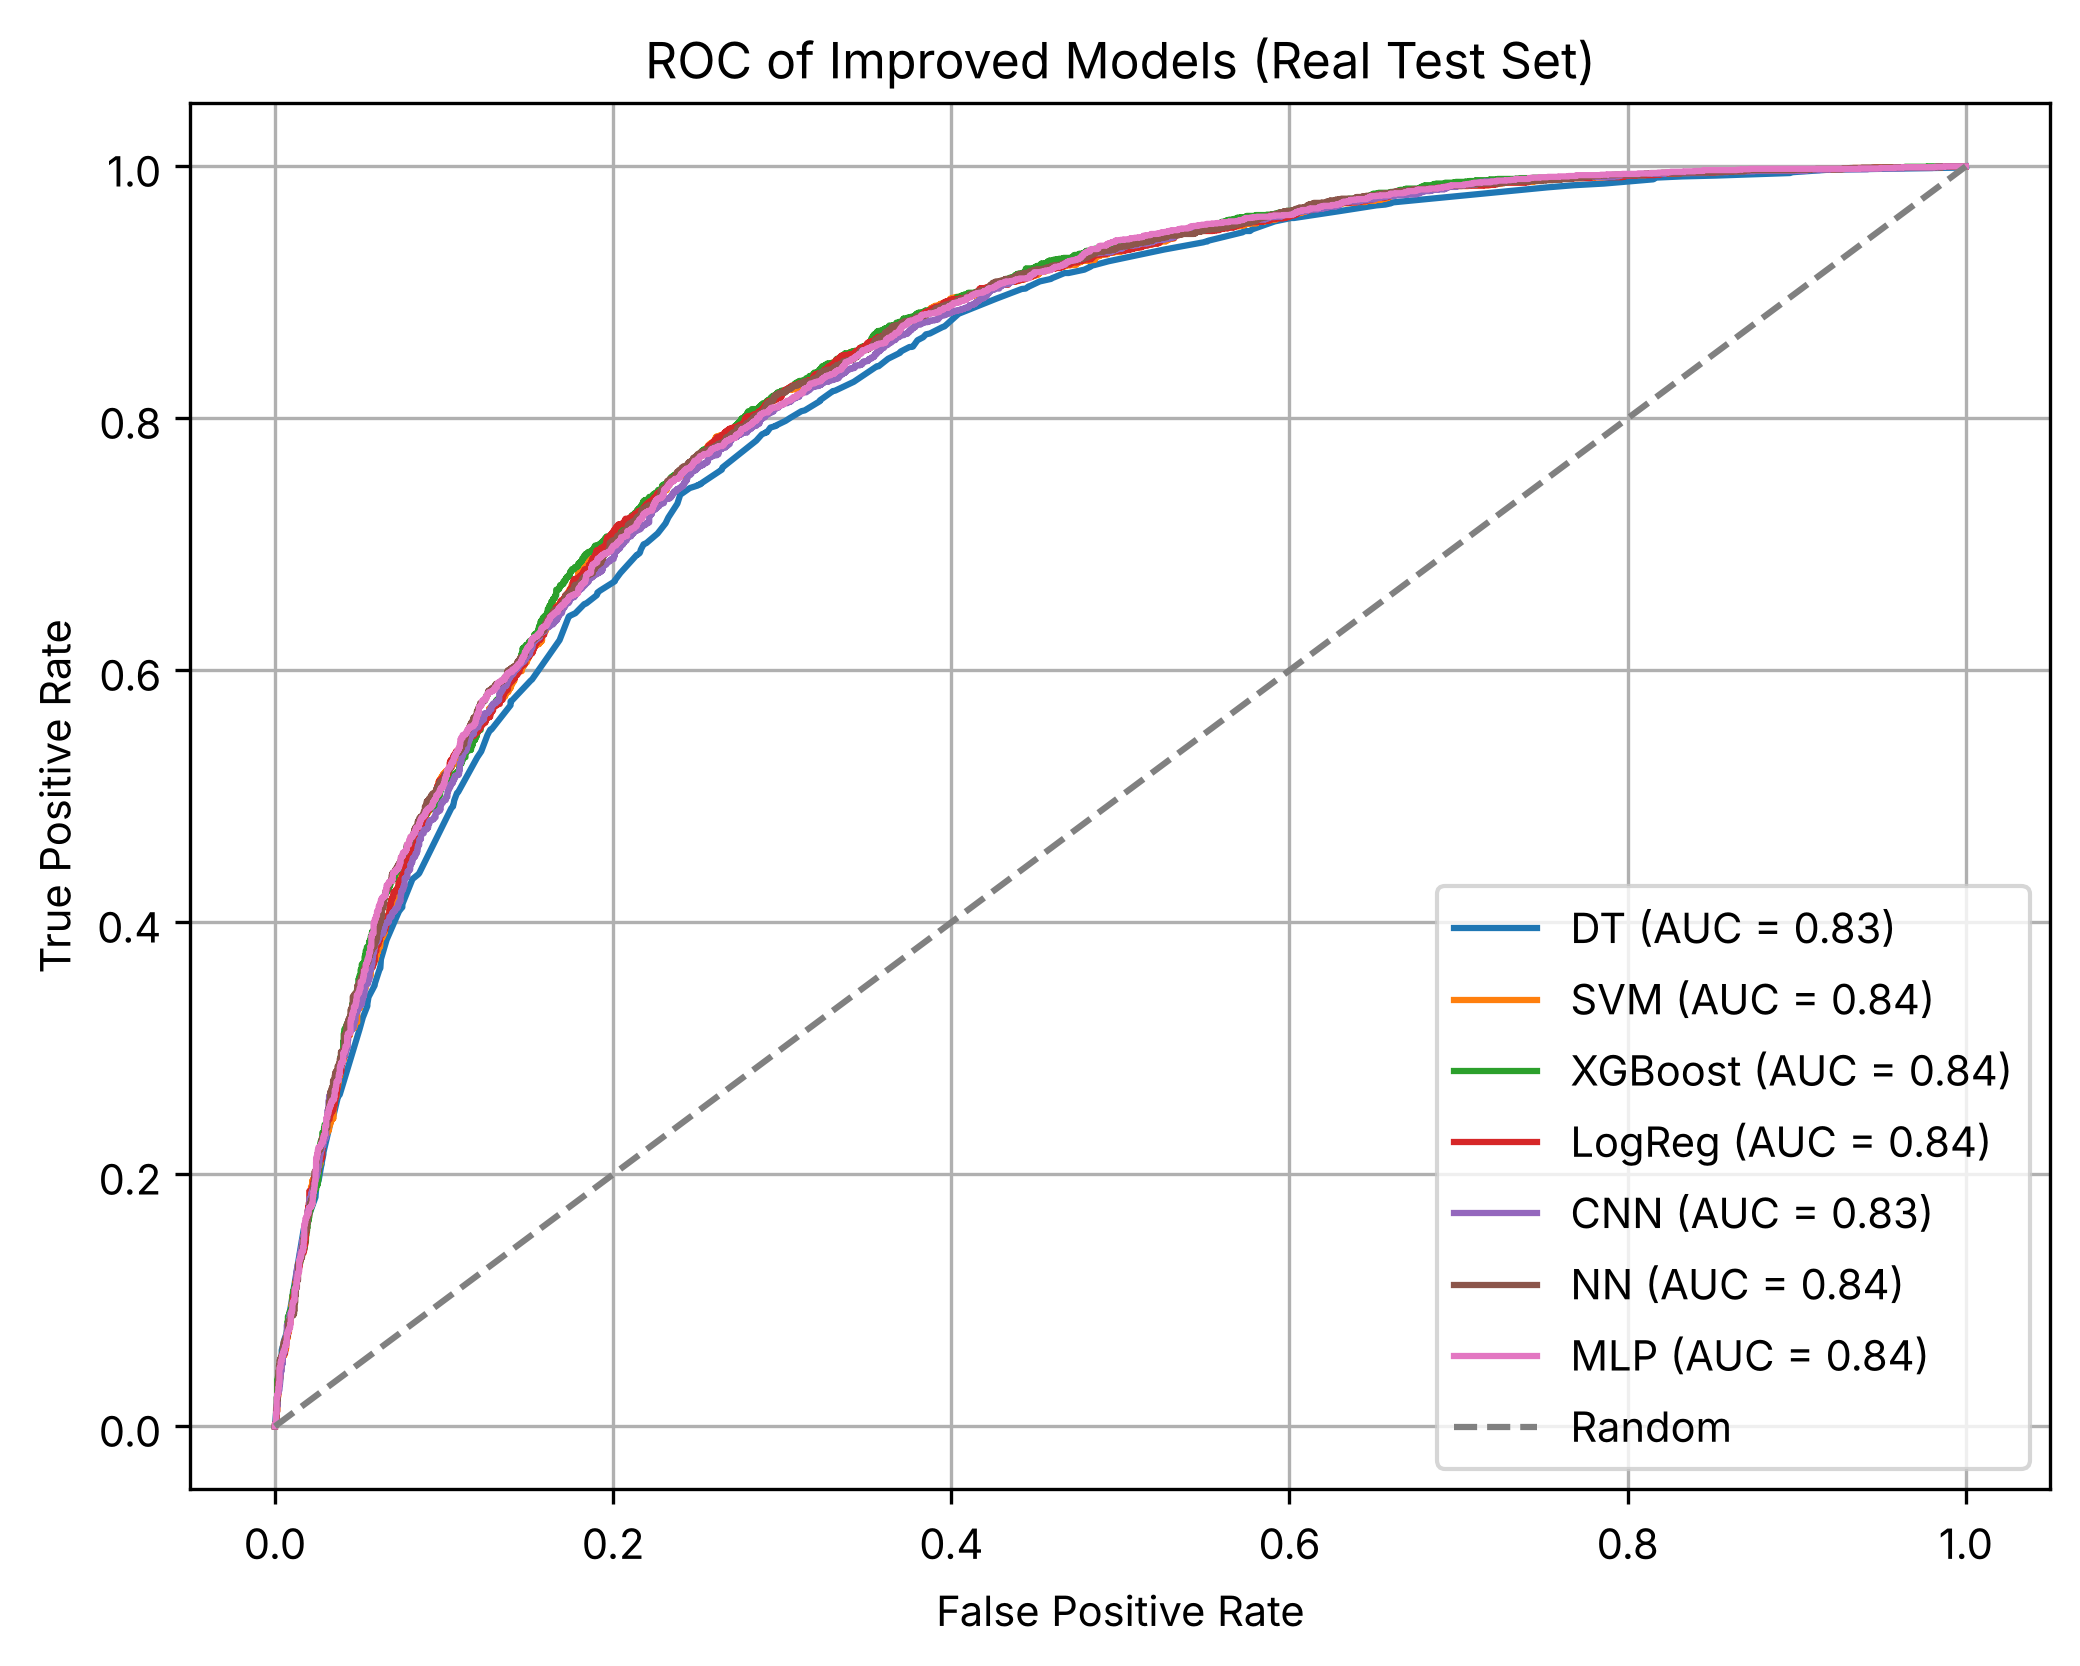
\includegraphics[width=0.6\linewidth]{figures/roc_improved.png}
\caption{ROC curves of the improved models on the real, unseen test set
(Protocol B).}
\label{fig:rocB}
\end{figure}

\begin{figure}[t]
\centering
\begin{subfigure}{0.32\linewidth}
  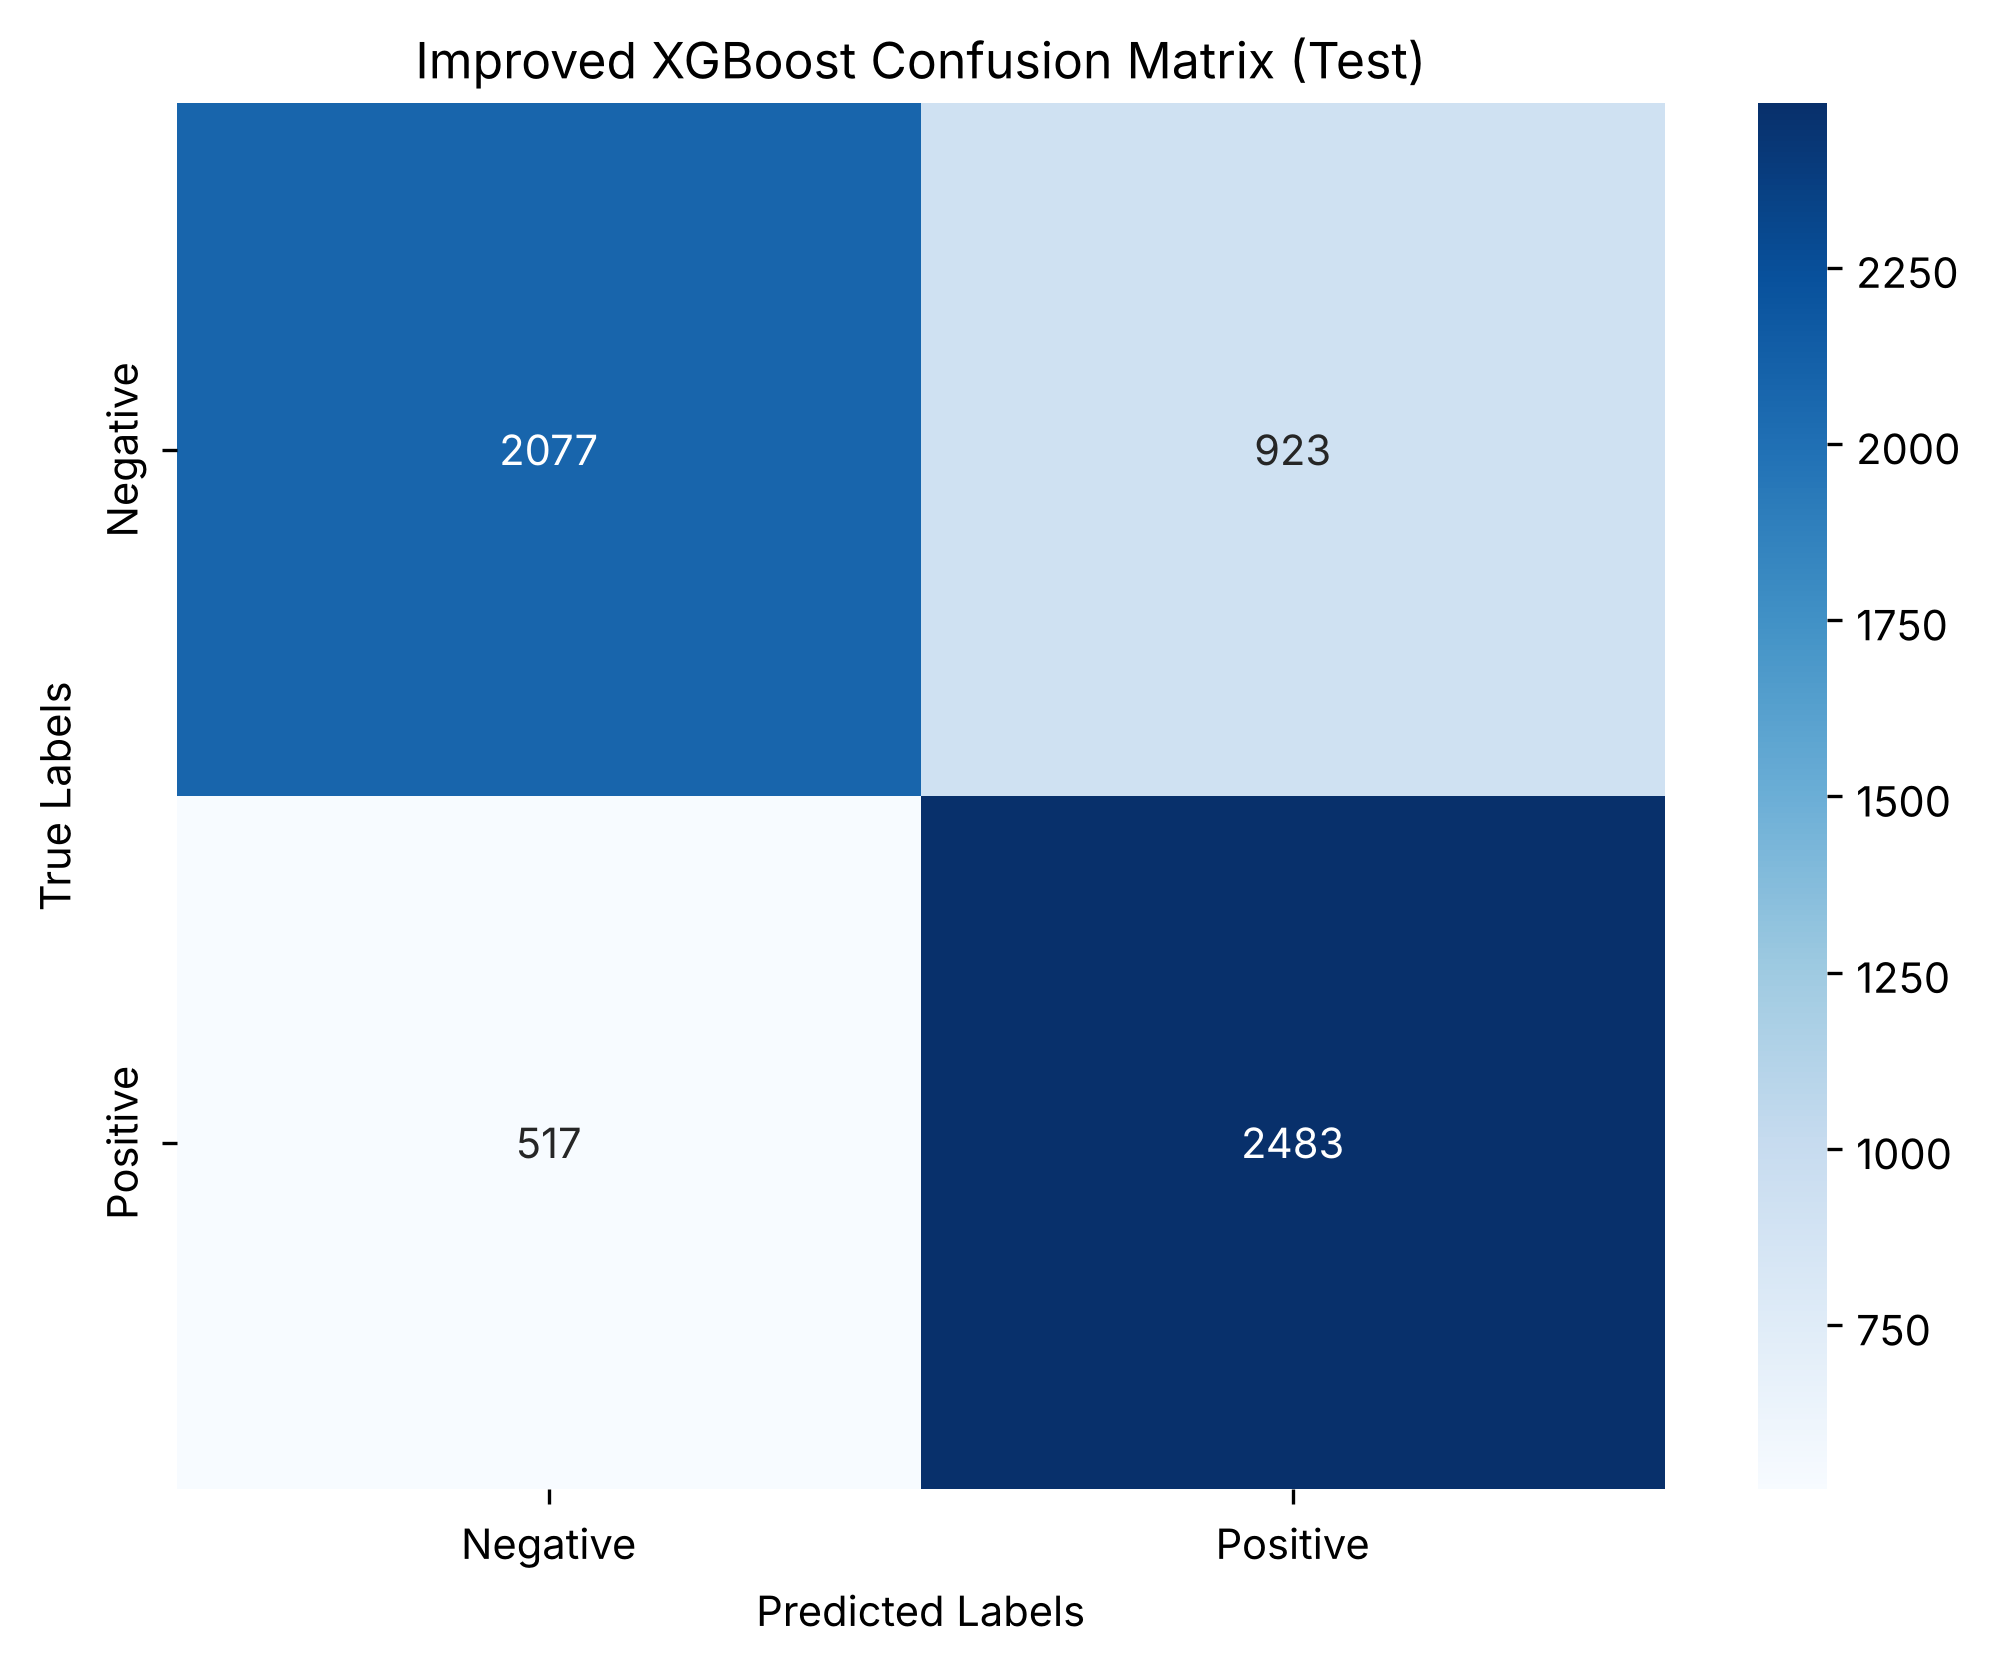
\includegraphics[width=\linewidth]{figures/improved_confusion_matrix_XGBoost.png}
  \caption{XGBoost}
\end{subfigure}
\begin{subfigure}{0.32\linewidth}
  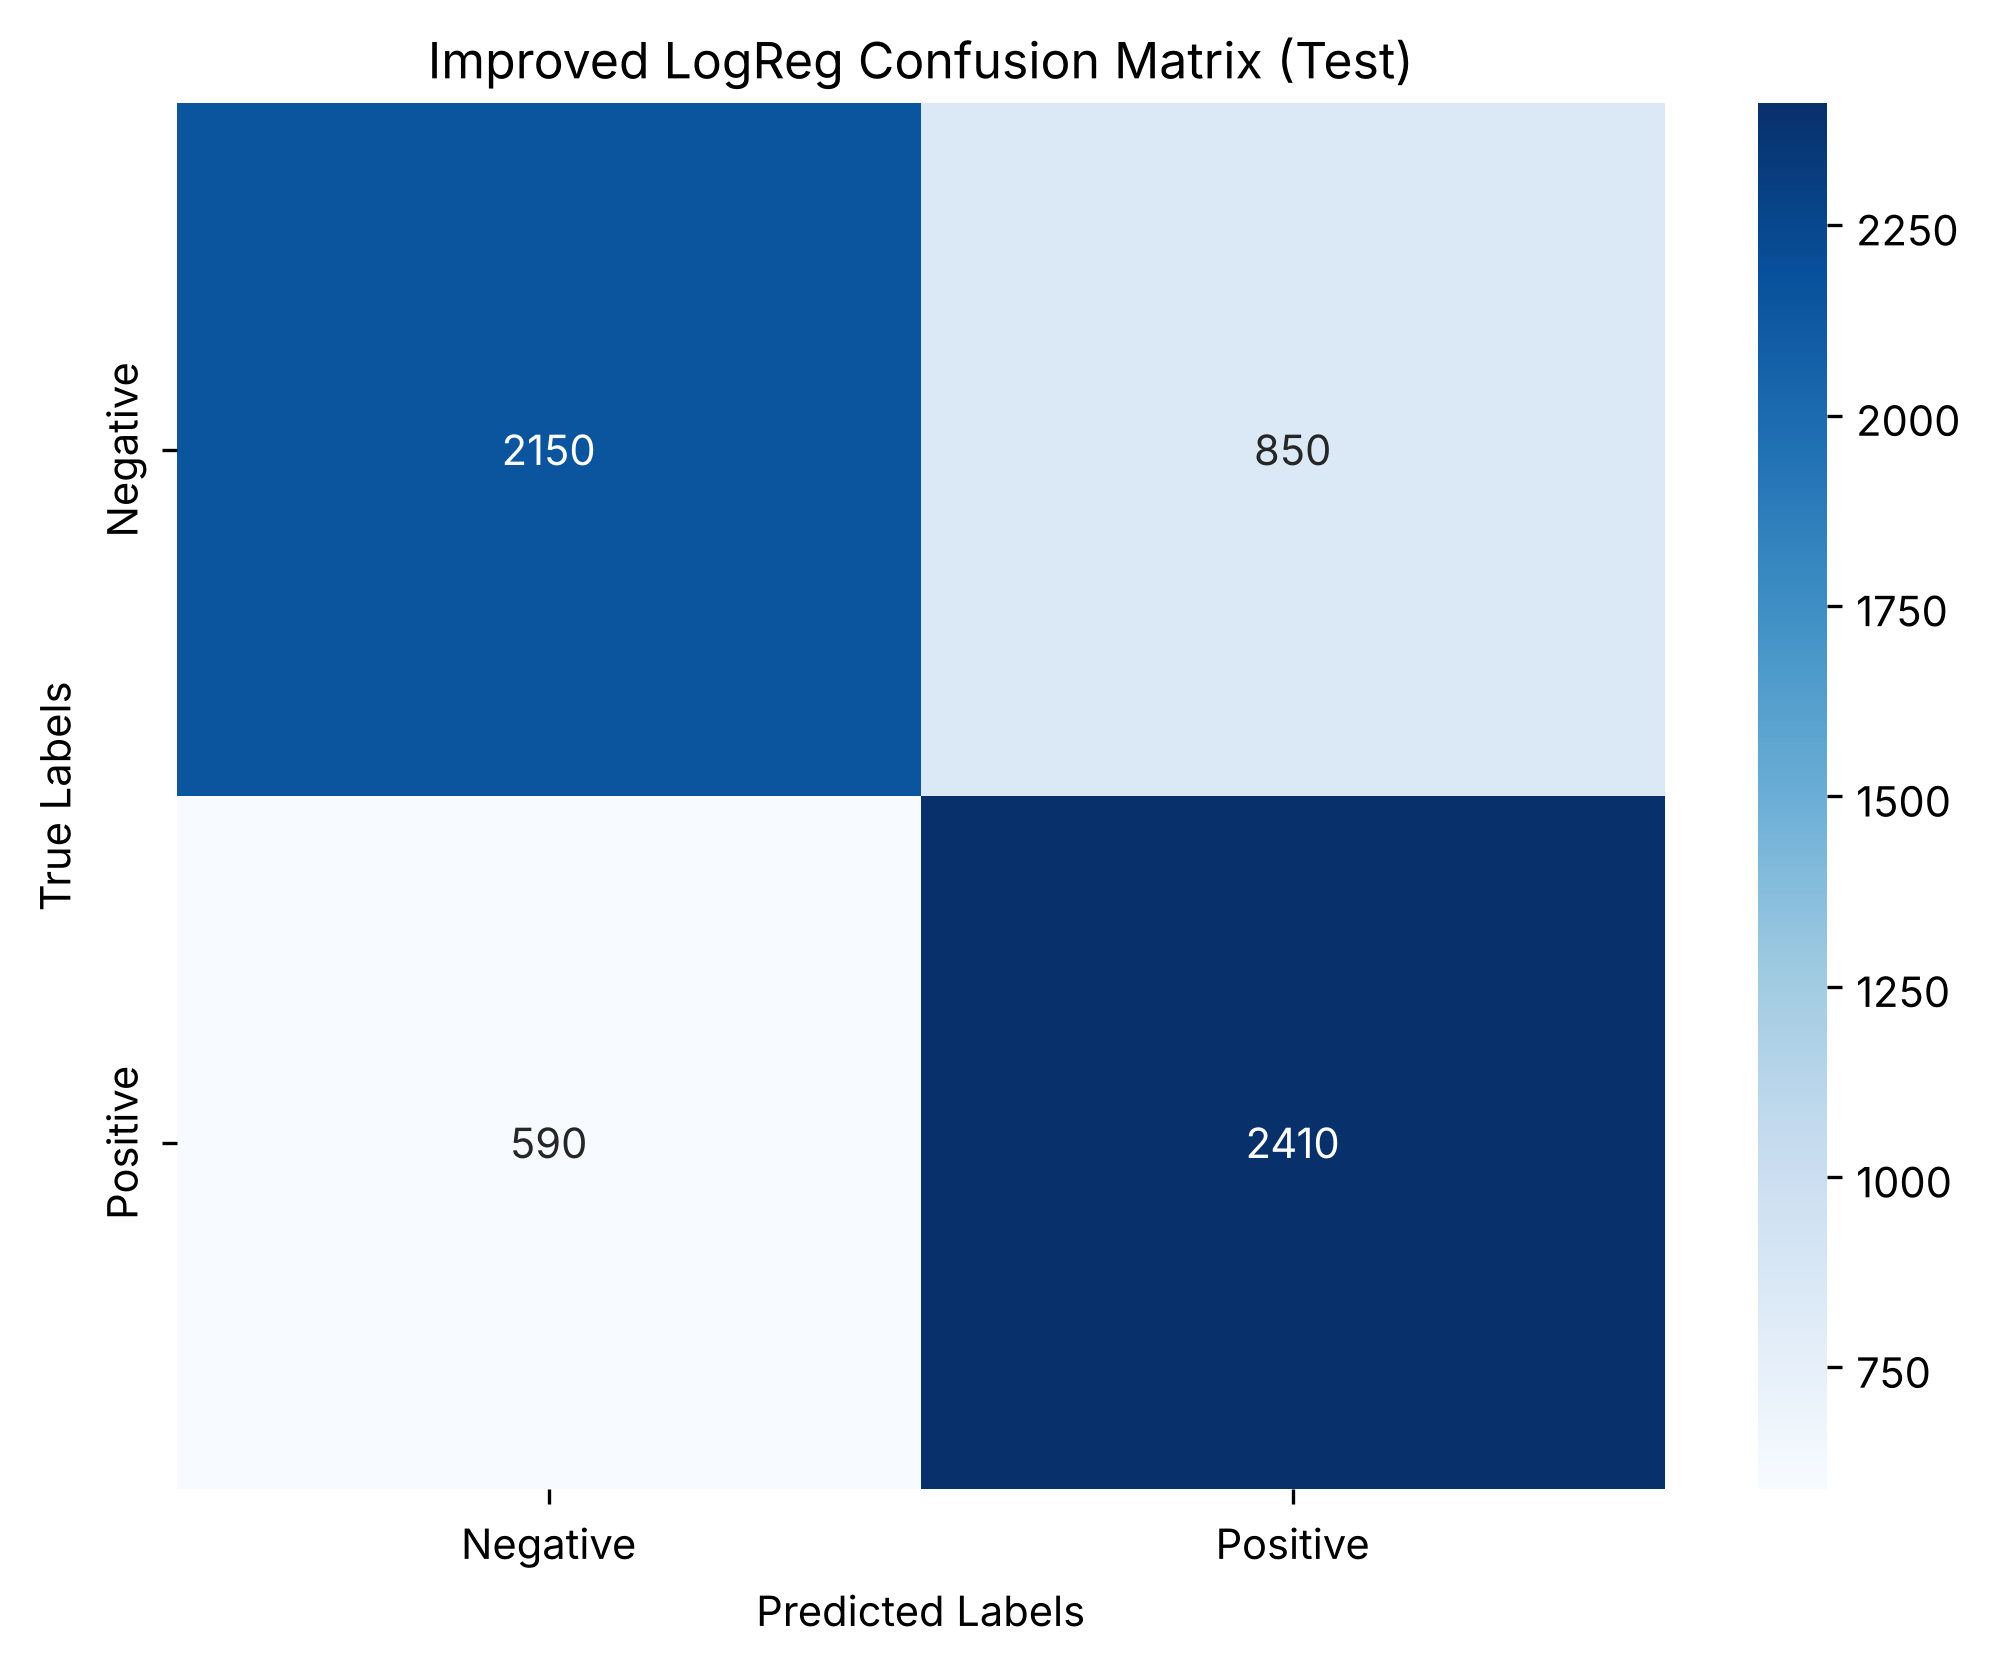
\includegraphics[width=\linewidth]{figures/improved_confusion_matrix_LogReg.png}
  \caption{Logistic regression}
\end{subfigure}
\begin{subfigure}{0.32\linewidth}
  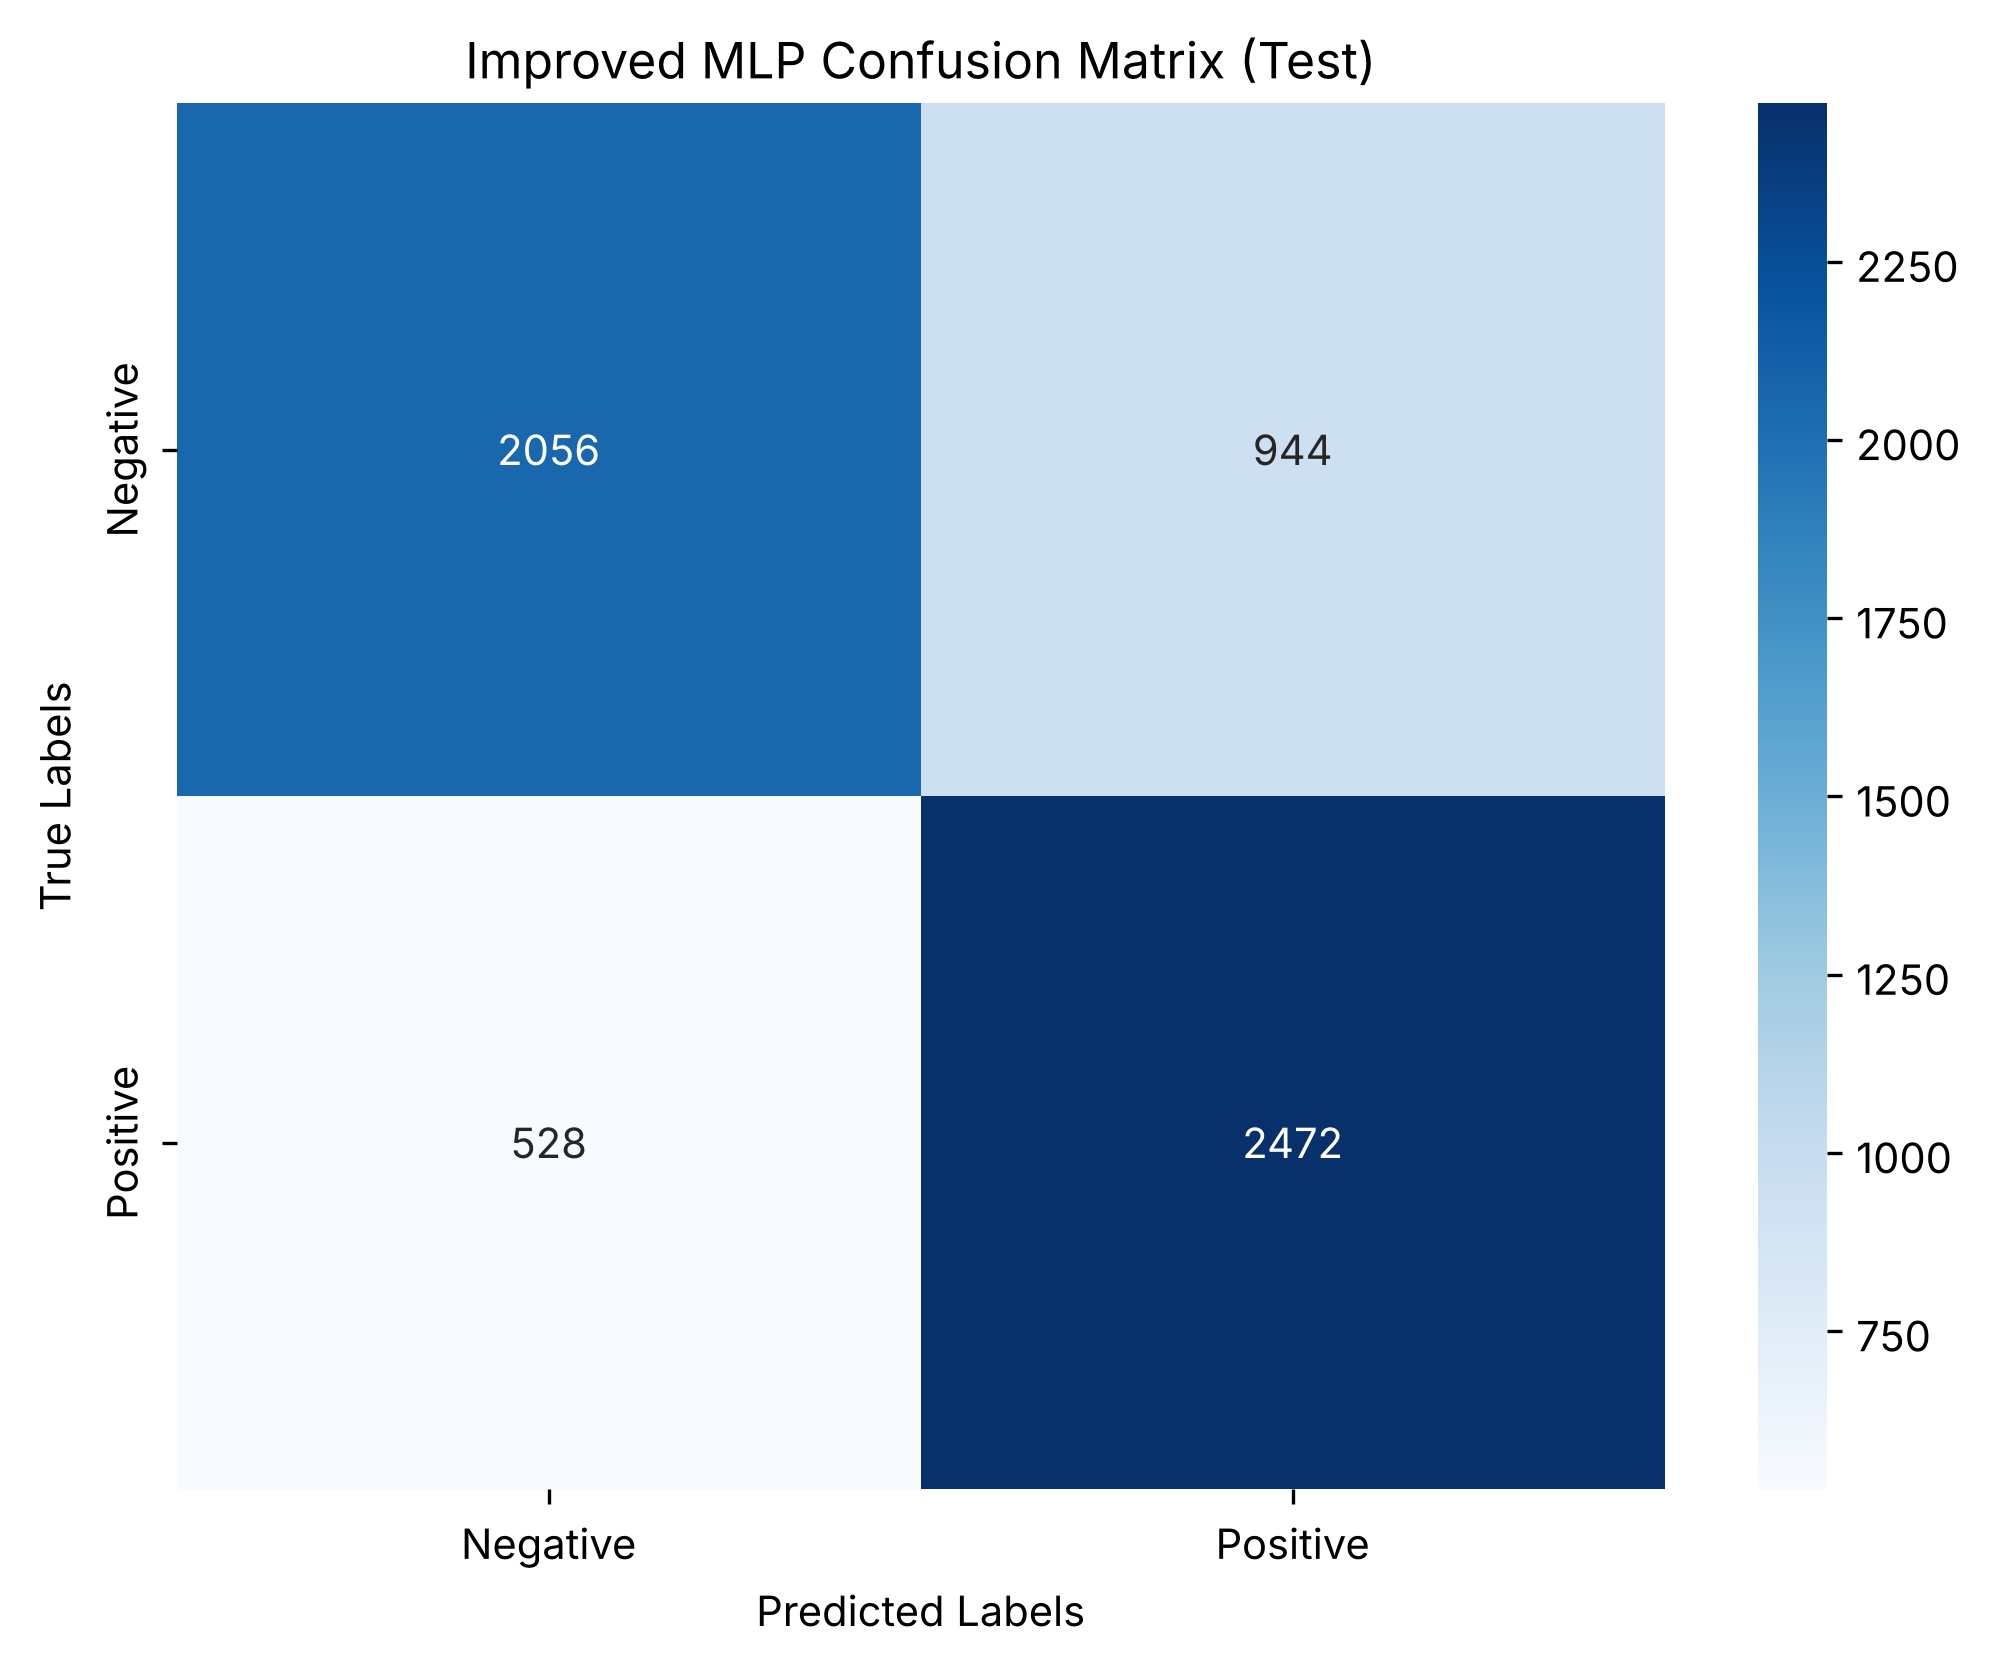
\includegraphics[width=\linewidth]{figures/improved_confusion_matrix_MLP.png}
  \caption{MLP}
\end{subfigure}
\caption{Confusion matrices of improved models on the real test set
(Protocol B, 3,000 records per class).}
\label{fig:cmB}
\end{figure}

\begin{figure}[t]
\centering
\begin{subfigure}{\linewidth}
  \centering
  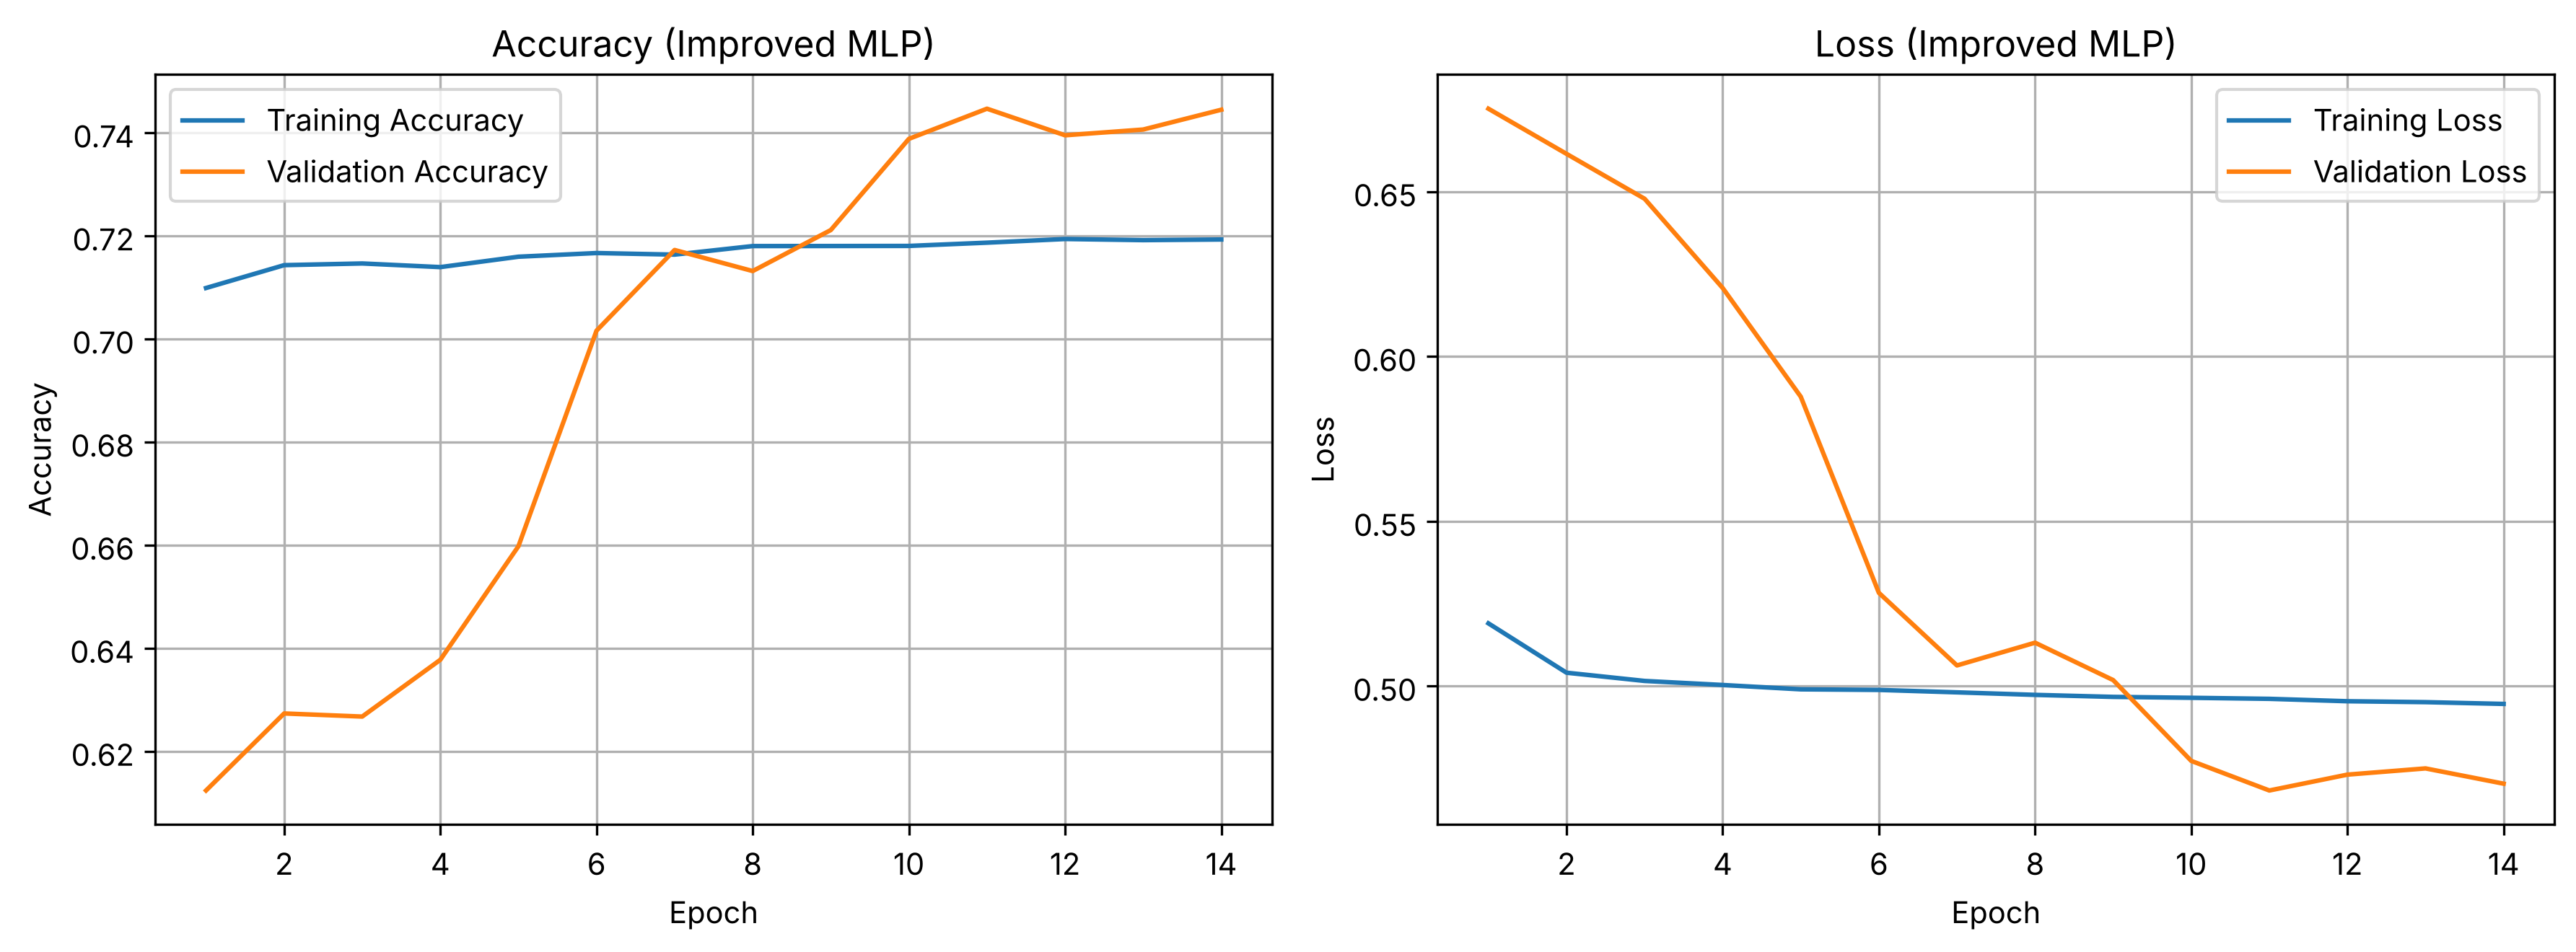
\includegraphics[width=0.85\linewidth]{figures/improved_learning_curve_MLP.png}
  \caption{MLP}
\end{subfigure}
\begin{subfigure}{\linewidth}
  \centering
  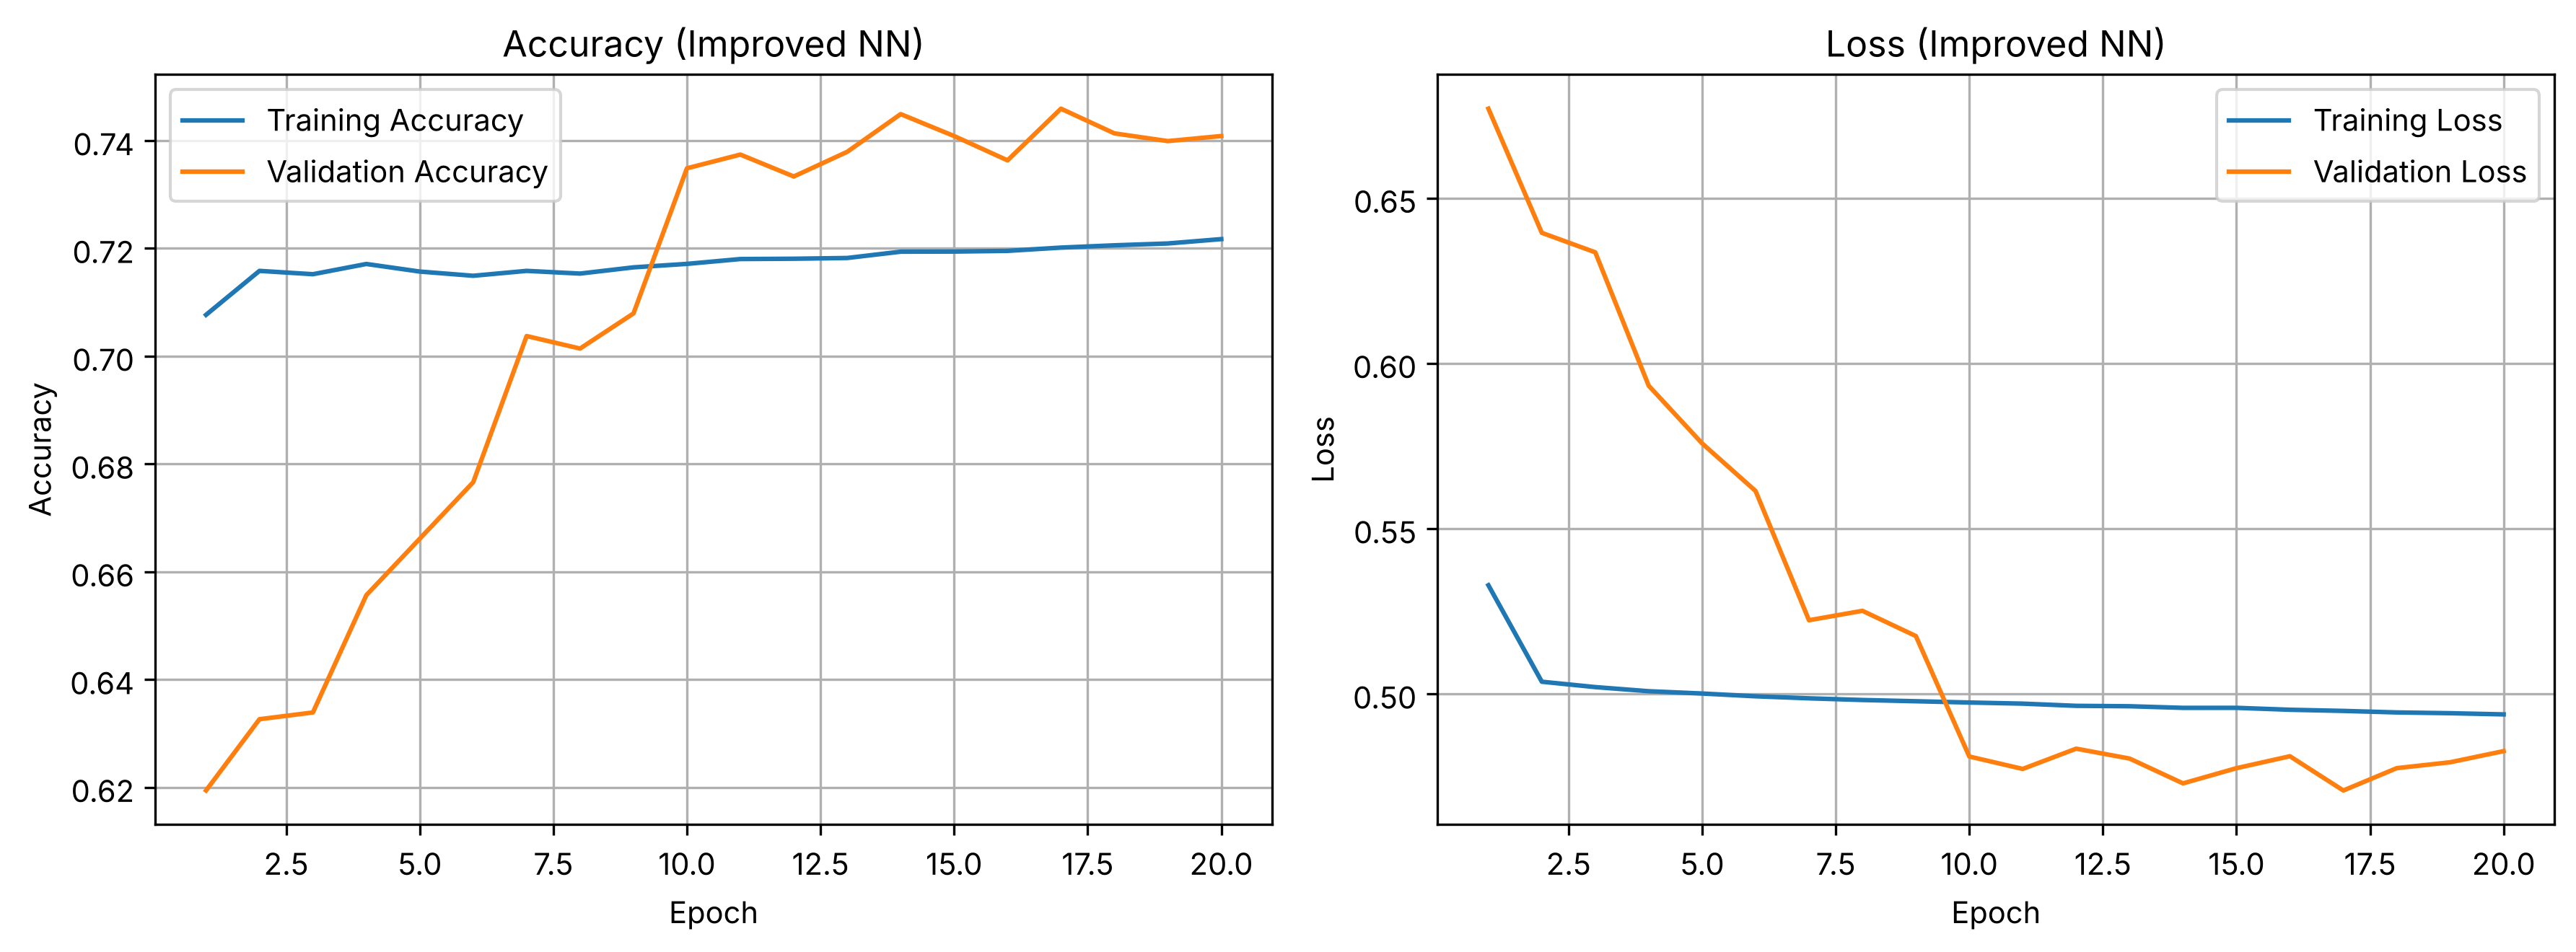
\includegraphics[width=0.85\linewidth]{figures/improved_learning_curve_NN.png}
  \caption{NN}
\end{subfigure}
\caption{Training and validation accuracy and loss of the improved DL
models; training stops early once the validation loss no longer
improves.}
\label{fig:lcB}
\end{figure}

\subsubsection{Five-fold cross-validation}
\label{sec:cv}

To check that these results do not depend on one particular split, the
improved models were evaluated with stratified five-fold cross-validation
on the 223,781 real records that are not in the test set. In every fold,
20\% of the training portion was set aside for early stopping and threshold
tuning, and the held-out fold kept the real prevalence of about 10.3\%.
Table~\ref{tab:cv} reports the mean and standard deviation over the folds.
The AUC (0.824--0.839) and recall (78.9--82.5\%) agree with the test-set
results and vary little between folds (standard deviation of the AUC at
most 0.64 percentage points), confirming that the estimates are stable.
Accuracy (70.8--72.2\%) is lower than on the balanced test set because the
tuned threshold trades specificity for sensitivity and negatives make up
almost 90\% of each fold.

\begin{table}[t]
\centering
\caption{Five-fold cross-validation of the improved models on real records
at the natural prevalence of CVD (about 10.3\%); mean $\pm$ standard
deviation over the folds, in \%.}
\label{tab:cv}
\small
\begin{tabular}{lccccc}
\toprule
Model & Accuracy & Precision & Recall & F1 Score & AUC \\
\midrule
\inputrows{tables/cv_improved.tex}
\bottomrule
\end{tabular}
\end{table}

Precision and F1 are much lower in cross-validation than on the balanced
test set because the folds keep the real prevalence. At a prevalence of
10\%, even a model with about 80\% sensitivity and 70\% specificity flags
roughly three to four healthy respondents for every true CVD case
(precision about 22\%). This is an inherent property of screening for a
condition of low prevalence, not a defect of a particular model, and it
should guide how such models are used: as inexpensive pre-screening tools
that refer at-risk individuals for clinical assessment, not as diagnostic
tests.

\subsection{Comparison with Existing Studies}
\label{sec:compare}

Table~\ref{tab:literature} compares the proposed method with existing
studies. With a few exceptions, previous studies achieved accuracy rates
between 82\% and 96\%, and studies on small datasets such as the Cleveland
heart disease data (303 records) report the highest values. These figures
are not directly comparable: the studies use different datasets with
different clinical variables, and several do not state whether resampling
or feature selection was performed before the data were split. Our results
show that this choice alone can change the reported accuracy of the same
model on the same data from 57\% to 99.8\%. For the proposed method we
therefore report the leakage-free results on 6,000 real BRFSS records. Of
the studies listed, Amarbayasgalan et al.~\cite{amarbayasgalan} used the
KNHANES survey (25,340 records), which is closest in nature to BRFSS.

\begin{table}[t]
\centering
\caption{Comparison of the proposed method with existing studies. The
proposed results are leakage-free (Protocol B, real held-out test set).}
\label{tab:literature}
\footnotesize
\setlength{\tabcolsep}{3pt}
\begin{tabular}{lllccccc}
\toprule
Study & Dataset & Method & Acc. (\%) & Prec. (\%) & Rec. (\%) & F1 (\%) & AUC (\%) \\
\midrule
M. Bhatt et al.~\cite{bhatt} & CVD dataset & XGBoost & 87.02 & 89.62 & 82.11 & 86.30 & 95.00 \\
S. K. Mohan et al.~\cite{mohan} & Cleveland & Hybrid (HRFLM) & 88.40 & 90.10 & 92.80 & 90.00 & -- \\
N. L. Fitriyani et al.~\cite{fitriyani} & Cleveland & SMOTEENN + XGBoost & 95.90 & 97.14 & 94.67 & 95.35 & -- \\
W. Chang et al.~\cite{chang} & Beijing dataset & Hybrid XGBSVM & 91.70 & -- & -- & -- & 93.90 \\
A. A. Almazroi et al.~\cite{almazroi} & Cleveland & DNN & 82.49 & -- & 87.24 & 84.41 & -- \\
J. P. Li et al.~\cite{li} & Cleveland & SVM (Linear) & 85.00 & -- & 75.00 & -- & -- \\
T. Amarbayasgalan et al.~\cite{amarbayasgalan} & KNHANES & Two DNNs & 89.20 & 91.10 & 92.00 & 91.50 & 97.54 \\
\midrule
Proposed (improved) & BRFSS & XGBoost & 76.00 & 72.90 & 82.77 & 77.52 & 83.99 \\
Proposed (improved) & BRFSS & Logistic regression & 76.00 & 73.93 & 80.33 & 77.00 & 83.70 \\
Proposed (improved) & BRFSS & MLP & 75.47 & 72.37 & 82.40 & 77.06 & 83.79 \\
\bottomrule
\end{tabular}
\end{table}

\subsection{Limitations}

The BRFSS data are self-reported and cross-sectional: the target records a
past diagnosis of coronary heart disease or myocardial infarction, so the
models identify individuals who resemble patients with a history of CVD
rather than predict future events. Self-reported survey answers also carry
less information than clinical measurements, which limits the attainable
discrimination. The models were developed and tested on a single survey
year without external validation, and the calibration of the predicted
probabilities was not assessed. The balanced test set makes accuracy
comparable across protocols, but precision and F1 depend on prevalence, and
the cross-validation results indicate the values to expect in a general
population.


\section{CONCLUSION AND FUTURE WORK}
\label{sec:conclusion}

This study combined hybrid sampling (SMOTEENN followed by ROS) with three
DL models (CNN, NN, MLP) and three classical ML models (DT, SVM, XGBoost)
for CVD prediction from the 2015 BRFSS survey, and evaluated them under two
protocols. When the full dataset is resampled before it is split, the
models report 94.7--99.8\% test accuracy. We showed that this performance
is an artefact of data leakage: every positive test record has an exact
copy in the training set, and the ENN step removes a fifth of the real
non-CVD records, the borderline cases, before the test set is drawn. On
6,000 real records held out before any sampling, the same models reach
only 57.4--70.8\% accuracy, and the fully grown decision tree that appeared
best falls to near chance level.

We therefore proposed a leakage-free pipeline that uses all available
features, handles class imbalance with class weights instead of synthetic
records, regularises the models and tunes the decision threshold on a
validation set. On real, unseen records it improves every model, to about
76\% accuracy, 80\% recall and an AUC of 0.84, values that five-fold
cross-validation confirms. The technical observations of this study are:

\begin{itemize}
  \item The evaluation protocol dominates the reported performance. Any
    resampling, cleaning or duplication must be applied after the test
    data have been set aside, and only to the training data; otherwise
    accuracy on imbalanced health data can be overstated by more than
    40 percentage points.
  \item On real data, hybrid sampling did not improve discrimination: it
    lowered the AUC of XGBoost from 0.823 to 0.743. Class weighting and a
    tuned decision threshold address imbalance without distorting the data.
  \item Correlation-based selection of nine features discarded useful
    information; using all 21 features raised the AUC.
  \item Model choice matters far less than data handling. Logistic
    regression, SVM, XGBoost and the three DL models all reach an AUC of
    0.83--0.84, so simple and interpretable models are a sound choice for
    this task.
  \item Compared on equal terms, the improved pipeline attains the highest
    AUC reported on the same BRFSS data (0.840), and applied unchanged to
    the clinical Cleveland data it reaches an AUC of about 0.90. Higher
    accuracies reported on clinical datasets largely reflect more
    informative clinical measurements and small, variable test sets, and
    cannot be taken as evidence of a better method without a comparable,
    leakage-free evaluation.
  \item At the real prevalence of about 10\%, a model that detects 80\% of
    CVD cases still produces three to four false alarms for every true case
    (precision about 22\%). Survey-based models are therefore suited to
    low-cost screening and risk stratification that triggers clinical
    follow-up, not to diagnosis.
\end{itemize}

Future work should validate the pipeline on external cohorts and later
BRFSS survey years, study the calibration of the predicted probabilities,
and add clinical measurements (for example blood pressure readings, lipid
profiles and ECG data), which are likely needed to move beyond the
performance ceiling of self-reported data. Explainability methods such as
SHAP values could make the models' risk factors transparent to clinicians,
and threshold selection could be aligned with the costs of missed cases
and false alarms in a specific screening programme. We also encourage
authors of CVD prediction studies to report the point at which resampling
is applied and to release their code, so that results can be verified and
compared.


\section*{CODE AND DATA AVAILABILITY}

The dataset used in this study is publicly available on
Kaggle~\cite{teboul} and in the GitHub repository at
\url{https://github.com/daniyalabdulah/Early-Detection-of-Heart-Disease-using-Deep-Learning}.
The complete source code, which reproduces every table and figure in this
paper, is available at
\url{https://github.com/mohsinkhan85/Biomedical-Neurocomputing-Lab}.

\section*{ACKNOWLEDGMENTS}

This work was supported by King Saud University, Riyadh, Saudi Arabia,
through Researchers Supporting Project number RSP2024R184.

\begin{thebibliography}{99}
\small

\bibitem{who} World Health Organization. Cardiovascular Diseases. Webpage, 2023. Available at: \url{https://www.who.int/health-topics/cardiovascular-diseases} (Accessed on June 23, 2023).

\bibitem{mathers} Colin D. Mathers and Dejan Loncar. Projections of global mortality and burden of disease from 2002 to 2030. \emph{PLoS Med}, 3(11):e442, 2006. doi: \href{https://doi.org/10.1371/journal.pmed.0030442}{10.1371/journal.pmed.0030442}.

\bibitem{mayo} Mayo Clinic. Heart disease. Webpage, 2019. Available at: \url{https://www.mayoclinic.org/diseases-conditions/heart-disease/symptoms-causes/syc-20353118} (Accessed on June 23, 2023).

\bibitem{libby} Peter Libby. Mechanisms of acute coronary syndromes and their implications for therapy. \emph{New England Journal of Medicine}, 368(21):2004--2013, 2013. doi: \href{https://doi.org/10.1056/NEJMra1216063}{10.1056/NEJMra1216063}.

\bibitem{yusuf} Salim Yusuf, Steven Hawken, Stephanie \^{O}unpuu, Tony Dans, Alvaro Avezum, Fernando Lanas, Matthew McQueen, Andrzej Budaj, Prem Pais, John Varigos, and Liu Lisheng. Effect of potentially modifiable risk factors associated with myocardial infarction in 52 countries (the INTERHEART study): Case-control study. \emph{The Lancet}, 364(9438):937--952, 2004. doi: \href{https://doi.org/10.1016/S0140-6736(04)17018-9}{10.1016/S0140-6736(04)17018-9}.

\bibitem{virani} Salim S. Virani, Alvaro Alonso, Eunsik J. Benjamin, Marcio S. Bittencourt, Clifton W. Callaway, April P. Carson, Alanna M. Chamberlain, Alexander R. Chang, Susan Cheng, Francesca N. Delling, et al. Heart disease and stroke statistics---2020 update: A report from the American Heart Association. \emph{Circulation}, 141(9):e139--e596, 2020. doi: \href{https://doi.org/10.1161/CIR.0000000000000757}{10.1161/CIR.0000000000000757}.

\bibitem{alaref} Subhi J. Al'Aref, Kimberly Anchouche, Gaurav Singh, Patricia J. Slomka, Krzysztof K. Kolli, Amit Kumar, Mohit Pandey, Gabriel Maliakal, Alexander R. van Rosendael, Ashley N. Beecy, et al. Clinical applications of machine learning in cardiovascular disease and its relevance to cardiac imaging. \emph{European Heart Journal}, 40(24):1975--1986, 2019. doi: \href{https://doi.org/10.1093/eurheartj/ehy404}{10.1093/eurheartj/ehy404}.

\bibitem{gavhane} Aditi Gavhane, Gouthami Kokkula, Isha Pandya, and Kailas Devadkar. Prediction of heart disease using machine learning. In \emph{2018 Second International Conference on Electronics, Communication and Aerospace Technology (ICECA)}, pages 1275--1278, 2018. doi: \href{https://doi.org/10.1109/ICECA.2018.8474922}{10.1109/ICECA.2018.8474922}.

\bibitem{sheikabdullah} A. SheikAbdullah. A data mining model to predict and analyze the events related to coronary heart disease using decision trees with particle swarm optimization for feature selection. \emph{International Journal of Computer Applications}, 55:49--55, 2012. doi: \href{https://doi.org/10.5120/8779-2736}{10.5120/8779-2736}.

\bibitem{currie} Geoffrey Currie, Kristina Hawk, Eric Rohren, Alanna Vial, and Ran Klein. Machine learning and deep learning in medical imaging: Intelligent imaging. \emph{Journal of Medical Imaging and Radiation Sciences}, 50, 2019. doi: \href{https://doi.org/10.1016/j.jmir.2019.09.005}{10.1016/j.jmir.2019.09.005}.

\bibitem{chlif} M. Chlif, N. M. Ammar, N. Ben Said, L. Sergey, S. Ahmaidi, F. Alassery, and H. Hamam. Mechanism of dyspnea during exercise in children with corrected congenital heart disease. \emph{Int. J. Environ. Res. Public Health}, 19(99), 2022. doi: \href{https://doi.org/10.3390/ijerph19010099}{10.3390/ijerph19010099}.

\bibitem{hussain} N. M. Hussain, A. U. Rehman, M. T. B. Othman, J. Zafar, H. Zafar, and H. Hamam. Accessing artificial intelligence for fetus health status using hybrid deep learning algorithm (AlexNet-SVM) on cardiotocographic data. \emph{Sensors}, 2022. doi: \href{https://doi.org/10.3390/s22145103}{10.3390/s22145103}.

\bibitem{khan} A. A. Khan, A. A. Laghari, M. Shafiq, O. Cheikhrouhou, W. Alhakami, H. Hamam, and Z. A. Shaikh. Healthcare ledger management: A blockchain and machine learning-enabled novel and secure architecture for medical industry. \emph{Human-centric Computing and Information Sciences}, 12, 2022. doi: \href{https://doi.org/10.22967/HCIS.2022.12.055}{10.22967/HCIS.2022.12.055}.

\bibitem{fernando} C. D. Fernando, P. T. Weerasinghe, and C. K. Walgampaya. Heart disease risk identification using machine learning techniques for a highly imbalanced dataset: a comparative study. \emph{KDU Journal of Multidisciplinary Studies}, 4(2), 2022. doi: \href{https://doi.org/10.4038/kjms.v4i2.50}{10.4038/kjms.v4i2.50}.

\bibitem{ishaq} Abid Ishaq, Saima Sadiq, Muhammad Umer, Saleem Ullah, Seyedali Mirjalili, Vaibhav Rupapara, and Michele Nappi. Improving the prediction of heart failure patients' survival using SMOTE and effective data mining techniques. \emph{IEEE Access}, 9:39707--39716, 2021. doi: \href{https://doi.org/10.1109/ACCESS.2021.3064084}{10.1109/ACCESS.2021.3064084}.

\bibitem{singh2015} Arpit Singh and Anuradha Purohit. A survey on methods for solving data imbalance problem for classification. \emph{International Journal of Computer Applications}, 127(15):37--41, 2015. doi: \href{https://doi.org/10.5120/ijca2015906677}{10.5120/ijca2015906677}.

\bibitem{batista} Gustavo Batista, Ronaldo Prati, and Maria-Carolina Monard. A study of the behavior of several methods for balancing machine learning training data. \emph{SIGKDD Explorations}, 6:20--29, 2004. doi: \href{https://doi.org/10.1145/1007730.1007735}{10.1145/1007730.1007735}.

\bibitem{ali} Liaqat Ali, Abdur Rahman, Aurangzeb Khan, MengChu Zhou, Adeeb Javeed, and Jude A. Onwuegbuzie. Efficient prediction of cardiovascular disease using machine learning algorithms with Relief and LASSO feature selection techniques. \emph{IEEE Access}, 9:24505--24522, 2021. doi: \href{https://doi.org/10.1109/ACCESS.2021.3053759}{10.1109/ACCESS.2021.3053759}.

\bibitem{li} Jian Ping Li, Amin Ul Haq, Salah Ud Din, Jalaluddin Khan, Asif Khan, and Abdus Saboor. Heart disease identification method using machine learning classification in e-healthcare. \emph{IEEE Access}, 8:107562--107582, 2020. doi: \href{https://doi.org/10.1109/ACCESS.2020.3001149}{10.1109/ACCESS.2020.3001149}.

\bibitem{fitriyani} Norma Latif Fitriyani, Muhammad Syafrudin, Ganjar Alfian, and Jongtae Rhee. HDPM: an effective heart disease prediction model for a clinical decision support system. \emph{IEEE Access}, 8:133034--133050, 2020. doi: \href{https://doi.org/10.1109/ACCESS.2020.3010511}{10.1109/ACCESS.2020.3010511}.

\bibitem{ahmad} Ghulab Nabi Ahmad, Hira Fatima, Shafi Ullah, Abdelaziz Salah Saidi, et al. Efficient medical diagnosis of human heart diseases using machine learning techniques with and without GridSearchCV. \emph{IEEE Access}, 10:80151--80173, 2022. doi: \href{https://doi.org/10.1109/ACCESS.2022.3165792}{10.1109/ACCESS.2022.3165792}.

\bibitem{ramesh} T. R. Ramesh, Umesh Kumar Lilhore, M. Poongodi, Sarita Simaiya, Amandeep Kaur, and Mounir Hamdi. Predictive analysis of heart diseases with machine learning approaches. \emph{Malaysian Journal of Computer Science}, pages 132--148, 2022. doi: \href{https://doi.org/10.22452/mjcs.sp2022no1.10}{10.22452/mjcs.sp2022no1.10}.

\bibitem{qureshi} Muhammad Bilal Qureshi, Jason Glower, Daniel L. Ewert, and Steven C. Koenig. A novel idea to improve cardiac output of mechanical circulatory support devices by optimizing kinetic energy transfer available in forward moving aortic blood flow. \emph{Cardiovascular Engineering and Technology}, 8(2):131--144, 2017. doi: \href{https://doi.org/10.1007/s13239-017-0305-2}{10.1007/s13239-017-0305-2}.

\bibitem{azmi} Javed Azmi, Muhammad Arif, Md Tabrez Nafis, M. Afshar Alam, Safdar Tanweer, and Guojun Wang. A systematic review on machine learning approaches for cardiovascular disease prediction using medical big data. \emph{Medical Engineering \& Physics}, page 103825, 2022. doi: \href{https://doi.org/10.1016/j.medengphy.2022.103825}{10.1016/j.medengphy.2022.103825}.

\bibitem{singh2022} Vijendra Singh, Vijayan K. Asari, and Rajkumar Rajasekaran. A deep neural network for early detection and prediction of chronic kidney disease. \emph{Diagnostics}, 12(1), 2022. doi: \href{https://doi.org/10.3390/diagnostics12010116}{10.3390/diagnostics12010116}.

\bibitem{singhjain} Vijendra Singh and Divya Jain. A hybrid parallel classification model for the diagnosis of chronic kidney disease. \emph{International Journal of Interactive Multimedia and Artificial Intelligence}, 2021. doi: \href{https://doi.org/10.9781/ijimai.2021.10.008}{10.9781/ijimai.2021.10.008}.

\bibitem{jain2019} Divya Jain and Vijendra Singh. A two-phase hybrid approach using feature selection and adaptive SVM for chronic disease classification. \emph{International Journal of Computers and Applications}, 43:1--13, 2019. doi: \href{https://doi.org/10.1080/1206212X.2019.1577534}{10.1080/1206212X.2019.1577534}.

\bibitem{jain2020} Divya Jain and Vijendra Singh. A novel hybrid approach for chronic disease classification. \emph{International Journal of Healthcare Information Systems and Informatics (IJHISI)}, 15(1):1--19, 2020. doi: \href{https://doi.org/10.4018/IJHISI.2020010101}{10.4018/IJHISI.2020010101}.

\bibitem{mohan} Senthilkumar Mohan, Chandrasegar Thirumalai, and Gautam Srivastava. Effective heart disease prediction using hybrid machine learning techniques. \emph{IEEE Access}, 7:81542--81554, 2019. doi: \href{https://doi.org/10.1109/ACCESS.2019.2923707}{10.1109/ACCESS.2019.2923707}.

\bibitem{kavitha} M. Kavitha, G. Gnaneswar, R. Dinesh, Y. Rohith Sai, and R. Sai Suraj. Heart disease prediction using hybrid machine learning model. In \emph{2021 6th International Conference on Inventive Computation Technologies (ICICT)}, pages 1329--1333, 2021. doi: \href{https://doi.org/10.1109/ICICT50816.2021.9358597}{10.1109/ICICT50816.2021.9358597}.

\bibitem{teboul} Alex Teboul. Heart Disease Health Indicators Dataset. 2015. \url{https://www.kaggle.com/datasets/alexteboul/heart-disease-health-indicators-dataset}.

\bibitem{brfss} Centers for Disease Control and Prevention (CDC). Behavioral Risk Factor Surveillance System (BRFSS), 2022. Available at: \url{https://www.kaggle.com/datasets/cdc/behavioral-risk-factor-surveillance-system?select=2015.csv}.

\bibitem{brfsscalc} Centers for Disease Control and Prevention (CDC). Calculated variables in the 2015 data file of the BRFSS, 2015. Available at: \url{https://www.cdc.gov/brfss/annual_data/2015/pdf/2015_Calculated_Variables_Version4_08_10_17-508c.pdf} (Version 4, 08/10/17).

\bibitem{ullah2022} Zahid Ullah and Mona Jamjoom. An intelligent approach for Arabic handwritten letter recognition using convolutional neural network. \emph{PeerJ Computer Science}, 8:e995, 2022. doi: \href{https://doi.org/10.7717/peerj-cs.995}{10.7717/peerj-cs.995}.

\bibitem{ullah2023} Zahid Ullah and Mona Jamjoom. A deep learning for Alzheimer's stages detection using brain images. \emph{Computers, Materials and Continua}, 74, 2022. doi: \href{https://doi.org/10.32604/cmc.2023.032752}{10.32604/cmc.2023.032752}.

\bibitem{bhatt} Chintan M. Bhatt, Parth Patel, Tarang Ghetia, and Pier Luigi Mazzeo. Effective heart disease prediction using machine learning techniques. \emph{Algorithms}, 16(2), 2023. doi: \href{https://doi.org/10.3390/a16020088}{10.3390/a16020088}.

\bibitem{chang} Wenbing Chang, Yinglai Liu, Xueyi Wu, Yiyong Xiao, Shenghan Zhou, and Wen Cao. A new hybrid XGBSVM model: Application for hypertensive heart disease. \emph{IEEE Access}, 7:175248--175258, 2019. doi: \href{https://doi.org/10.1109/ACCESS.2019.2957367}{10.1109/ACCESS.2019.2957367}.

\bibitem{almazroi} Abdulwahab Ali Almazroi, Eman A. Aldhahri, Saba Bashir, and Sufyan Ashfaq. A clinical decision support system for heart disease prediction using deep learning. \emph{IEEE Access}, 11:61646--61659, 2023. doi: \href{https://doi.org/10.1109/ACCESS.2023.3285247}{10.1109/ACCESS.2023.3285247}.

\bibitem{amarbayasgalan} Tsatsral Amarbayasgalan, Van-Huy Pham, Nipon Theera-Umpon, Yongjun Piao, and Keun Ho Ryu. An efficient prediction method for coronary heart disease risk based on two deep neural networks trained on well-ordered training datasets. \emph{IEEE Access}, 9:135210--135223, 2021. doi: \href{https://doi.org/10.1109/ACCESS.2021.3116974}{10.1109/ACCESS.2021.3116974}.

\bibitem{kaufman} Shachar Kaufman, Saharon Rosset, Claudia Perlich, and Ori Stitelman. Leakage in data mining: Formulation, detection, and avoidance. \emph{ACM Transactions on Knowledge Discovery from Data}, 6(4):15:1--15:21, 2012. doi: \href{https://doi.org/10.1145/2382577.2382579}{10.1145/2382577.2382579}.

\bibitem{kapoor} Sayash Kapoor and Arvind Narayanan. Leakage and the reproducibility crisis in machine-learning-based science. \emph{Patterns}, 4(9):100804, 2023. doi: \href{https://doi.org/10.1016/j.patter.2023.100804}{10.1016/j.patter.2023.100804}.

\bibitem{santos} Miriam Seoane Santos, Jastin Pompeu Soares, Pedro Henriques Abreu, H\'{e}lder Ara\'{u}jo, and Jo\~{a}o Santos. Cross-validation for imbalanced datasets: avoiding overoptimistic and overfitting approaches. \emph{IEEE Computational Intelligence Magazine}, 13(4):59--76, 2018.

\bibitem{deng} Lang Deng, Kongjie Lu, and Huanhuan Hu. An interpretable LightGBM model for predicting coronary heart disease: Enhancing clinical decision-making with machine learning. \emph{PLOS ONE}, 20(9):e0330377, 2025. doi: \href{https://doi.org/10.1371/journal.pone.0330377}{10.1371/journal.pone.0330377}.

\bibitem{hasnat} Md Abrar Hasnat, Md Jobayer, Md. Mehedi Hasan Shawon, and Md. Golam Rabiul Alam. Interpretable heart disease prediction via a weighted ensemble model: A large-scale study with SHAP and surrogate decision trees. \emph{arXiv preprint arXiv:2511.01947}, 2025.

\bibitem{detrano} Andras Janosi, William Steinbrunn, Matthias Pfisterer, and Robert Detrano. Heart Disease [Dataset]. UCI Machine Learning Repository, 1989. doi: \href{https://doi.org/10.24432/C52P4X}{10.24432/C52P4X}.

\bibitem{pmlb} Randal S. Olson, William La Cava, Patryk Orzechowski, Ryan J. Urbanowicz, and Jason H. Moore. PMLB: a large benchmark suite for machine learning evaluation and comparison. \emph{BioData Mining}, 10:36, 2017. doi: \href{https://doi.org/10.1186/s13040-017-0154-4}{10.1186/s13040-017-0154-4}.

\end{thebibliography}


\end{document}
